%++++++++++++++++++++++++++++++++++++++++
% Don't modify this section unless you know what you're doing!
\documentclass[letterpaper,12pt]{article}
\usepackage{tabularx} % extra features for tabular environment
\usepackage{amsmath}  % improve math presentation
\usepackage{graphicx} % takes care of graphic including machinery
\usepackage[margin=1in,letterpaper]{geometry} % decreases margins
\usepackage[final]{hyperref} % adds hyper links inside the generated pdf file
\usepackage[utf8]{inputenc}
\usepackage{placeins}

\hypersetup{
	colorlinks=true,       % false: boxed links; true: colored links
	linkcolor=blue,        % color of internal links
	filecolor=magenta,     % color of file links
	urlcolor=blue         
}
%++++++++++++++++++++++++++++++++++++++++


\begin{document}

\title{Assignment 2}
\author{Ali Yeşilkanat - 2017700159}
\date{\today}
\maketitle

% \begin{abstract}
% In this experiment we studied a very important physical effect by measuring the
% dependence of a quantity $V$ of the quantity $X$ for two different sample
% temperatures.  Our experimental measurements confirmed the quadratic dependence
% $V = kX^2$ predicted by Someone's first law. The value of the mystery parameter
% $k = 15.4\pm 0.5$~s was extracted from the fit. This value is
% not consistent with the theoretically predicted $k_{theory}=17.34$~s. We attribute this
% discrepancy to low efficiency of our $V$-detector.
% \end{abstract}


\section{Introduction}

In this task, a basic image stitching system is developed to create a single panoramic image. 

\subsection{Select Common Points on Images}
Using matplotlib ginput function, user clicks common points for two images sequentially. In the code, clicked points are stored as variable and ginput function is commented in order to make experiments fast and consistent. Later on, common points pairs, used for homography estimation.

\subsection{Homography Estimation}
\subsubsection{Normalizing Points} \label{sssec:normalizing points}
Before homography estimation, points pairs are normalized for each corresponding image.
This is made by, calculating the average point of the points and assuming this point (centroid) as (0,0). Then, distance from centroid to the points is transformed to $\sqrt{2}$ by calculating normalizing matrix to make $\sqrt{2}$.

\subsubsection{Creating Homography Matrix}
In order to create homography matrix between two images, at least 4 points for each image has to be selected. If we call $n$ as the number selected points for an image, we need to create $2n X 9$ matrix equations.
\begin{center}
    

$p_i = \begin{bmatrix}
-x_i \quad -y_i \quad -1 \quad 0 \quad 0 \quad 0 \quad x_ix_i' \quad y_ix_i' \quad x_i' \\
0 \quad 0 \quad 0 \quad -x_i \quad -y_i \quad -1 \quad x_iy_i' \quad y_iy_i' \quad y_i'
\end{bmatrix}
$
\vspace{1em}
\newline
Then it is possible to stack all points into the matrix and solve $PH=0$ by SVD.
\newline
SVD $P = USV^\top$  select the last singular vector of V as the solution to H.
\vspace{250px}
\newline
Once we have H matrix, we can compute the projected coordinates of any point p(x,y) such as:

$\begin{bmatrix} \label{eq:hom_mul}
  x' / \lambda \\
  y' / \lambda \\
  \lambda
 \end{bmatrix} =
\begin{bmatrix}
  h_{11} & h_{12} & h_{13} \\
  h_{21} & h_{22} & h_{23} \\
  h_{31} & h_{32} & h_{33}
 \end{bmatrix}.
\begin{bmatrix}
  x \\
  y \\
  1
 \end{bmatrix}
$
\end{center}

\subsubsection{Denormalizing Points}
Using normalizing transform matrixes calculated in \ref{sssec:normalizing points} such that $T_1$ and $T_2$ for two images, calculated normalized homography matrix $\hat{H}$ is denormalized using equation:
\begin{center}
$ H= {T_2}^{-1} \hat{H} T_1$
\end{center}
\subsection{Image Warping}
By using calculated homography matrices for each image pairs, images stayed on both left and right of the center images are warped. 
Firstly reference points of image are calculated using homography matrix $H$ in order to learn new image shape after transformation. This is made by product of 4 corner points of the image and homography matrix \ref{eq:hom_mul}. 
\\
After deciding new image shape, all points of the image are traversed, and multiplied with homography matrix to find new coordinates. These y and x offsets are also subtracted from new $(y,x)$ coordinates of the image to fit image into new shape.
\subsection{Blending and Interpolation}
Not implemented. All warped images are projected sequentially into new image.
\section{Experiments}
All experiments are made using left-1, middle and right-1 images. Before doing experiments, common 12 points are selected using ginput. Later on, according to experiments' setup some of them used or some of them are changed randomly to create wrong matches. This is done for increasing speed in experiments.
\newpage
\subsection{Experiments with 5 points}
\subsubsection{5 Points Without Normalized Homography.}

\begin{figure}[!htb]
        \centering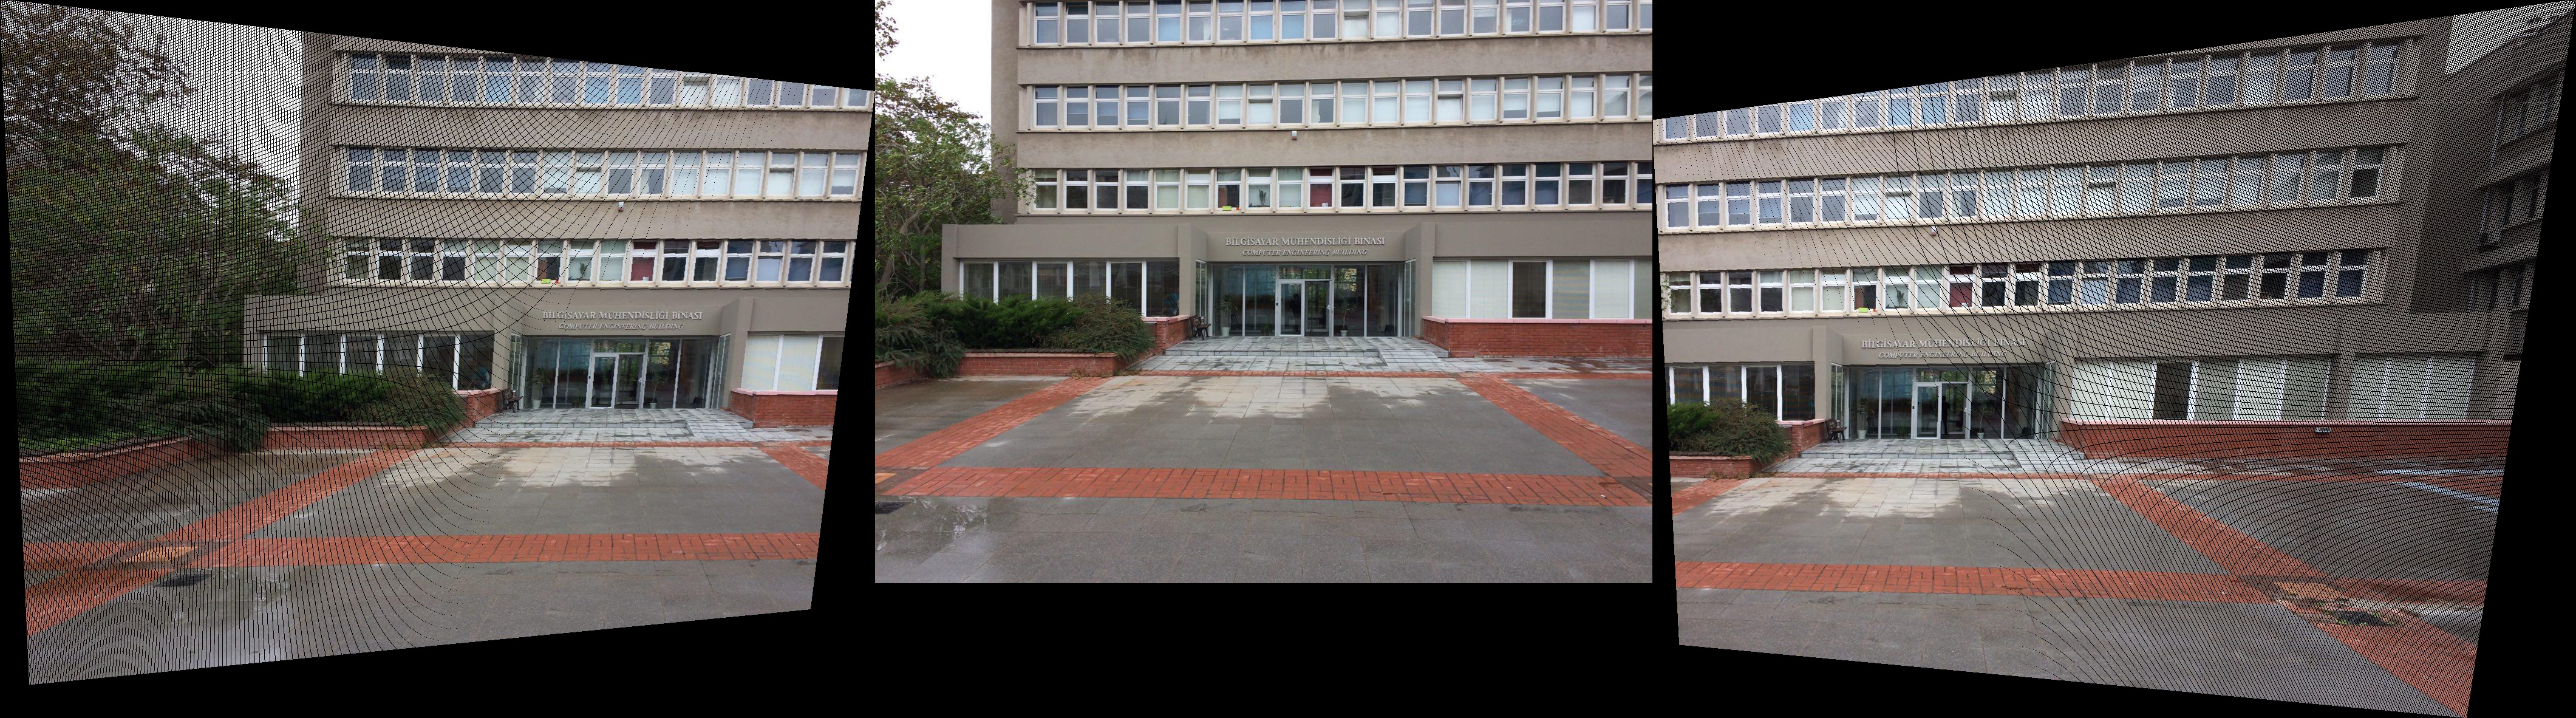
\includegraphics[width=1\columnwidth]{experiments/5points/finalNonewrong.jpg}
          \caption{
                \label{} Panoramic image
        }
        \centering\includegraphics[width=1\columnwidth]{experiments/5points/left-1_middleNonewrong.jpg}
          \caption{
                \label{} Common points between left and middle image.
        }
        \centering\includegraphics[width=1\columnwidth]{experiments/5points/middle_left-1Nonewrong.jpg}
        \caption{
                \label{} Common points between middle and right image.
        }
\end{figure}
\FloatBarrier
\newpage
\subsubsection{5 Points With Normalized Homography}
\begin{figure}[!htb]
        \centering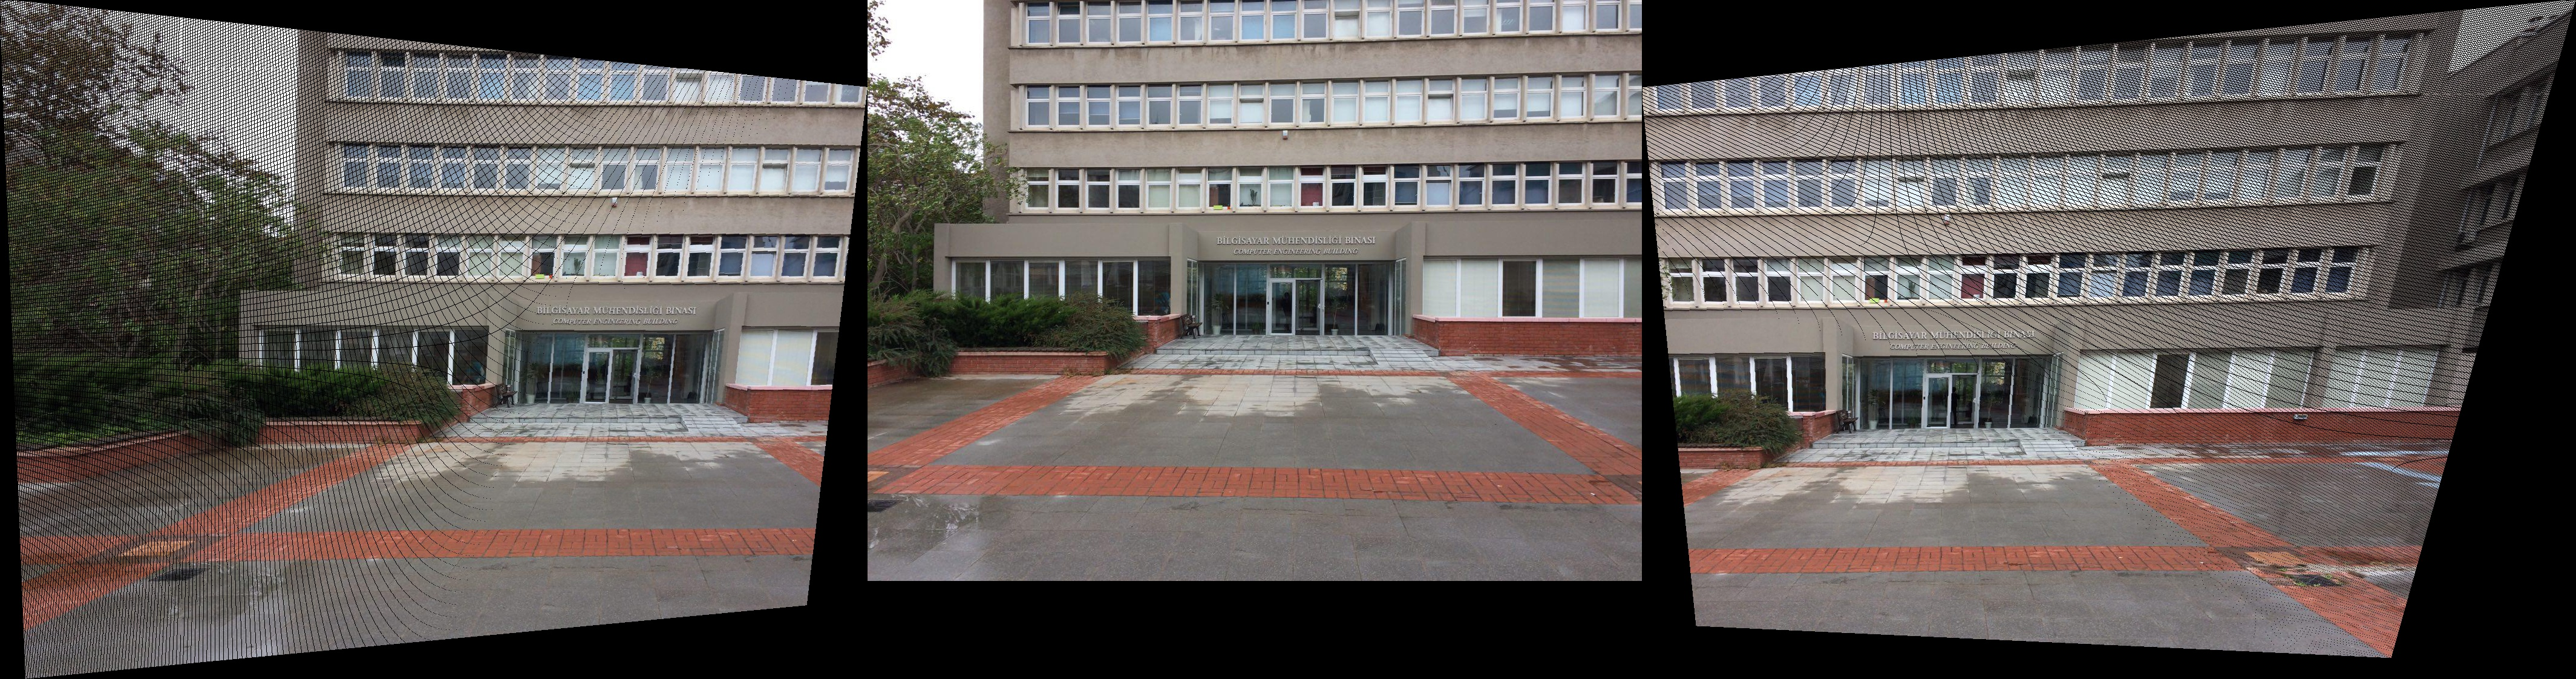
\includegraphics[width=1\columnwidth]{experiments/5points/norm/finalNonewrong.jpg}
          \caption{
                \label{} Panoramic image
        }
        \centering\includegraphics[width=1\columnwidth]{experiments/5points/norm/left-1_middleNonewrong.jpg}
          \caption{
                \label{} Common points between left and middle image.
        }
        \centering\includegraphics[width=1\columnwidth]{experiments/5points/norm/middle_left-1Nonewrong.jpg}
        \caption{
                \label{} Common points between middle and right image.
        }
\end{figure}

\FloatBarrier

\newpage
\subsubsection{5 Points with 3 Wrong Matches Without Normalized Homography.}

\begin{figure}[!htb]
        \centering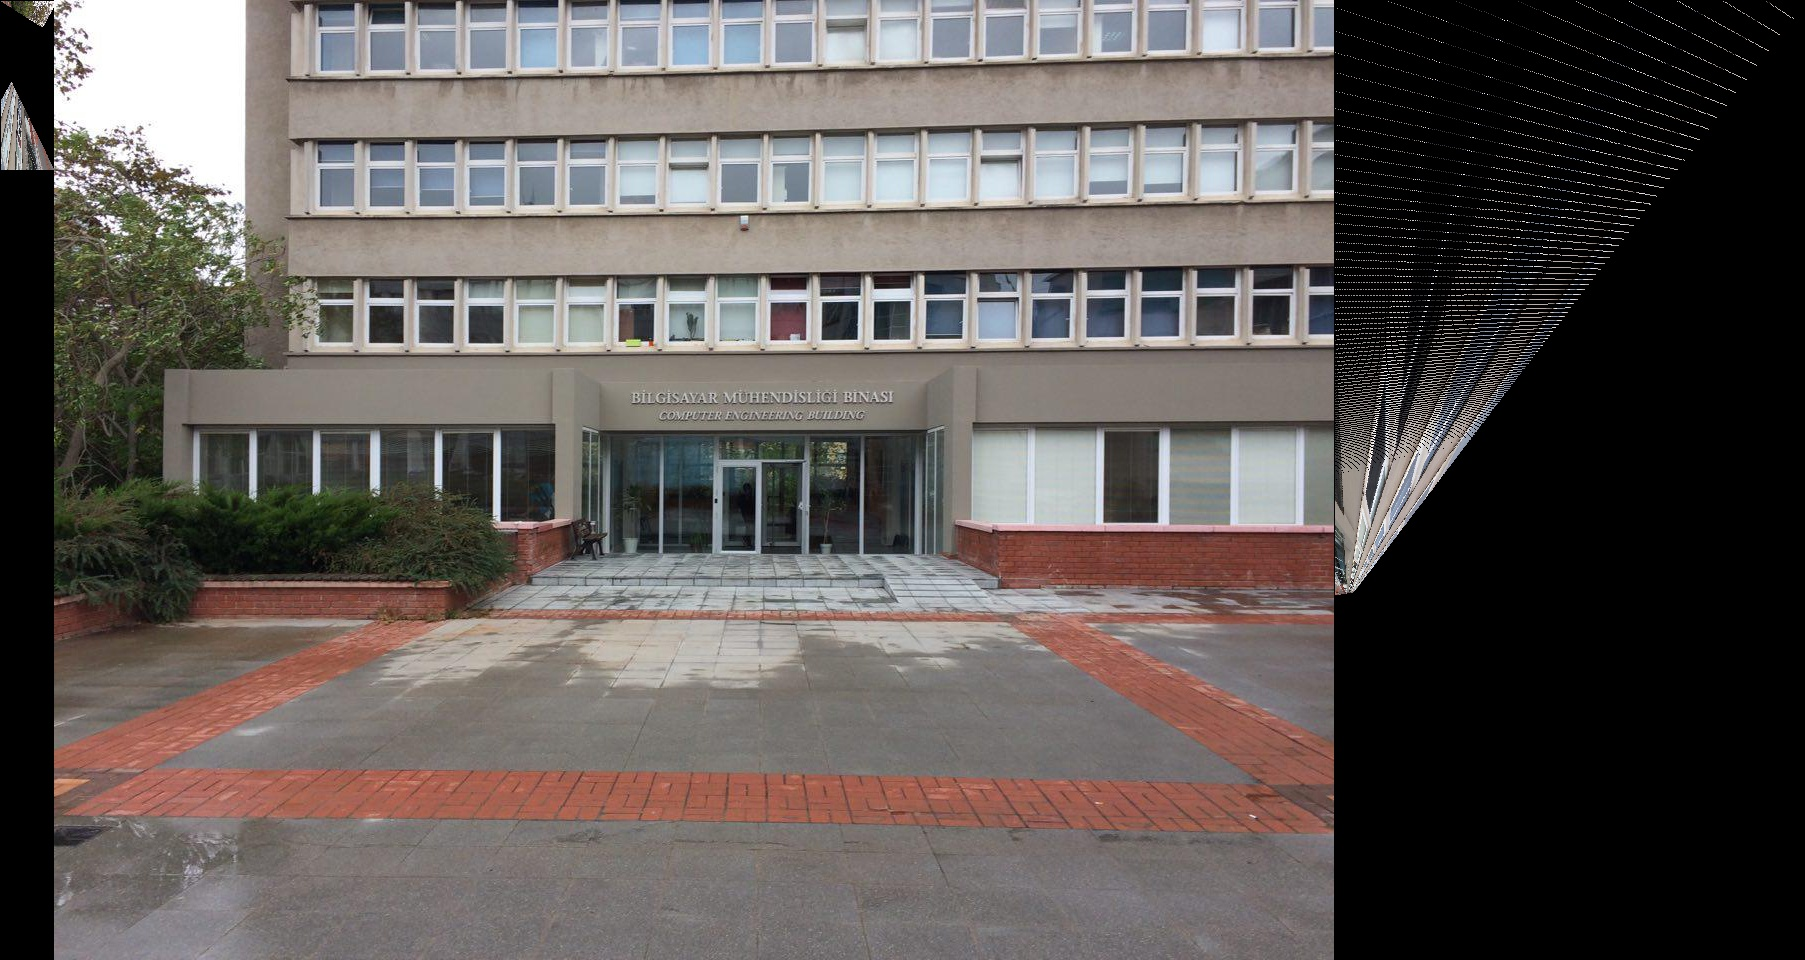
\includegraphics[width=1\columnwidth]{experiments/5points/final3wrong.jpg}
          \caption{
                \label{} Panoramic image
        }
        \centering\includegraphics[width=1\columnwidth]{experiments/5points/left-1_middle3wrong.jpg}
          \caption{
                \label{} Common points between left and middle image.
        }
        \centering\includegraphics[width=1\columnwidth]{experiments/5points/middle_left-13wrong.jpg}
        \caption{
                \label{} Common points between middle and right image.
        }
\end{figure}
\FloatBarrier
\newpage
\subsubsection{5 Points with 3 Wrong Matches With Normalized Homography.}
\begin{figure}[!htb]
        \centering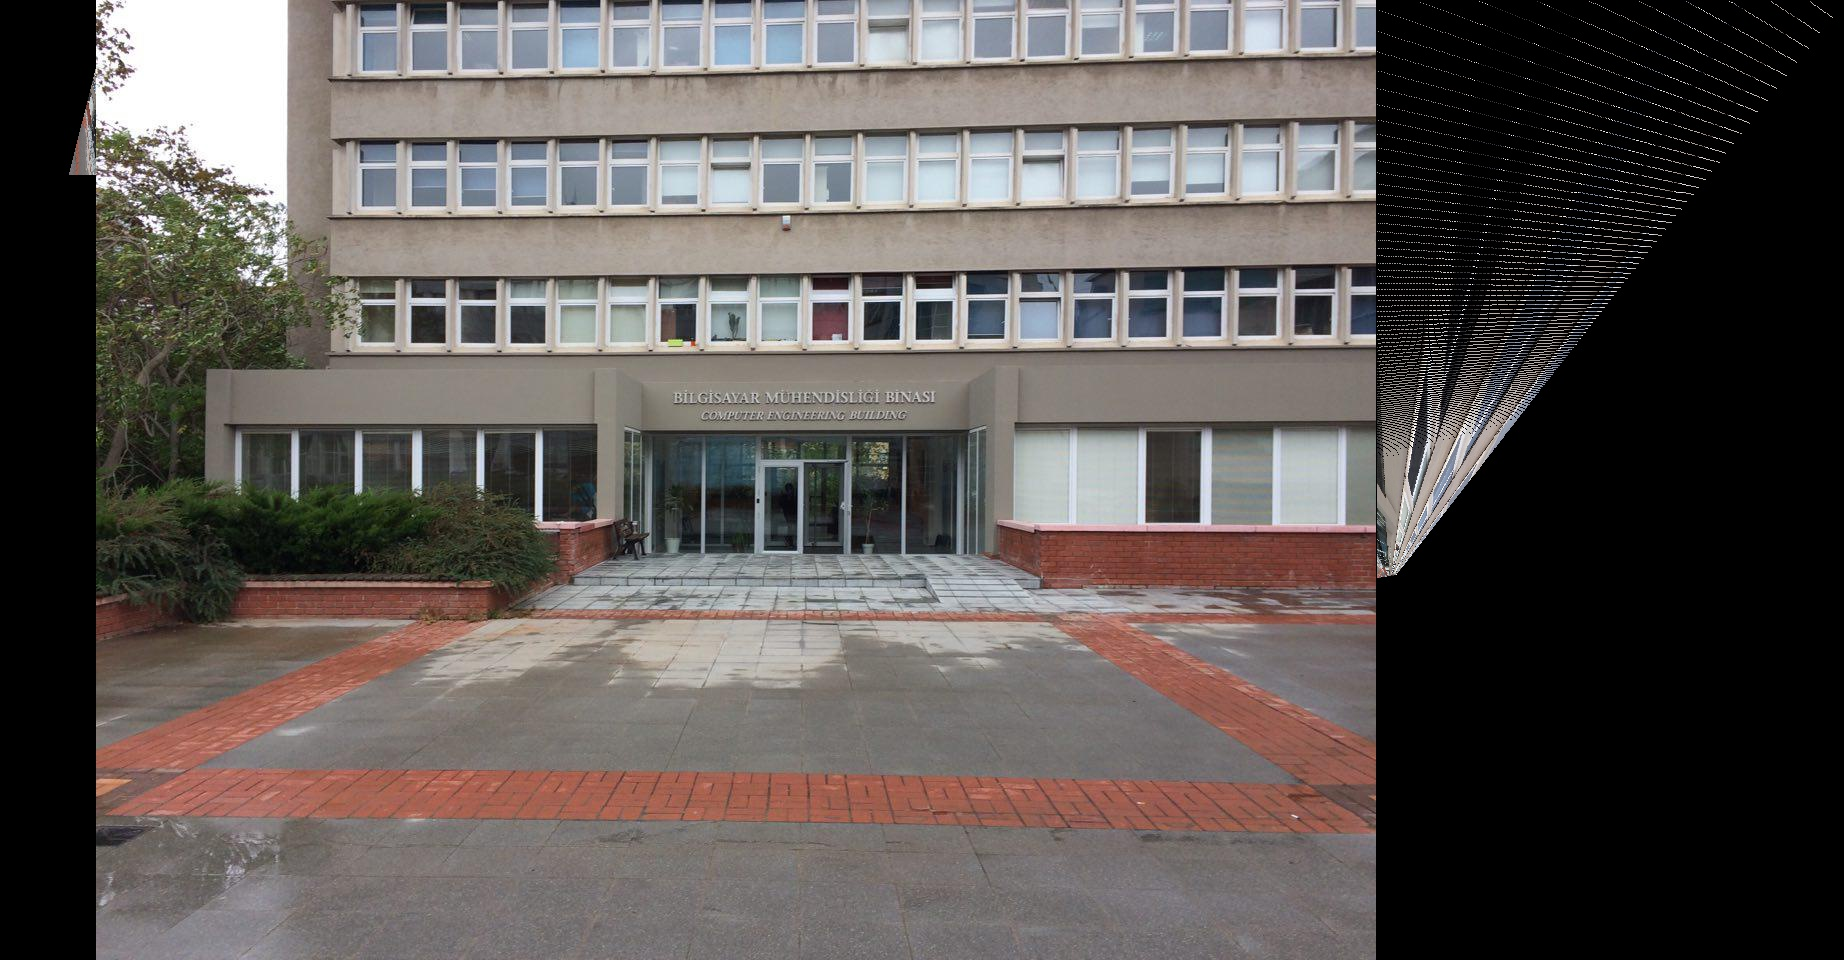
\includegraphics[width=1\columnwidth]{experiments/5points/norm/final3wrong.jpg}
          \caption{
                \label{} Panoramic image
        }
        \centering\includegraphics[width=1\columnwidth]{experiments/5points/norm/left-1_middle3wrong.jpg}
          \caption{
                \label{} Common points between left and middle image.
        }
        \centering\includegraphics[width=1\columnwidth]{experiments/5points/norm/middle_left-13wrong.jpg}
        \caption{
                \label{} Common points between middle and right image.
        }
\end{figure}
\FloatBarrier
\newpage
\subsubsection{5 Points with 5 Wrong Matches Without Normalized Homography.}
\begin{figure}[!htb]
        \centering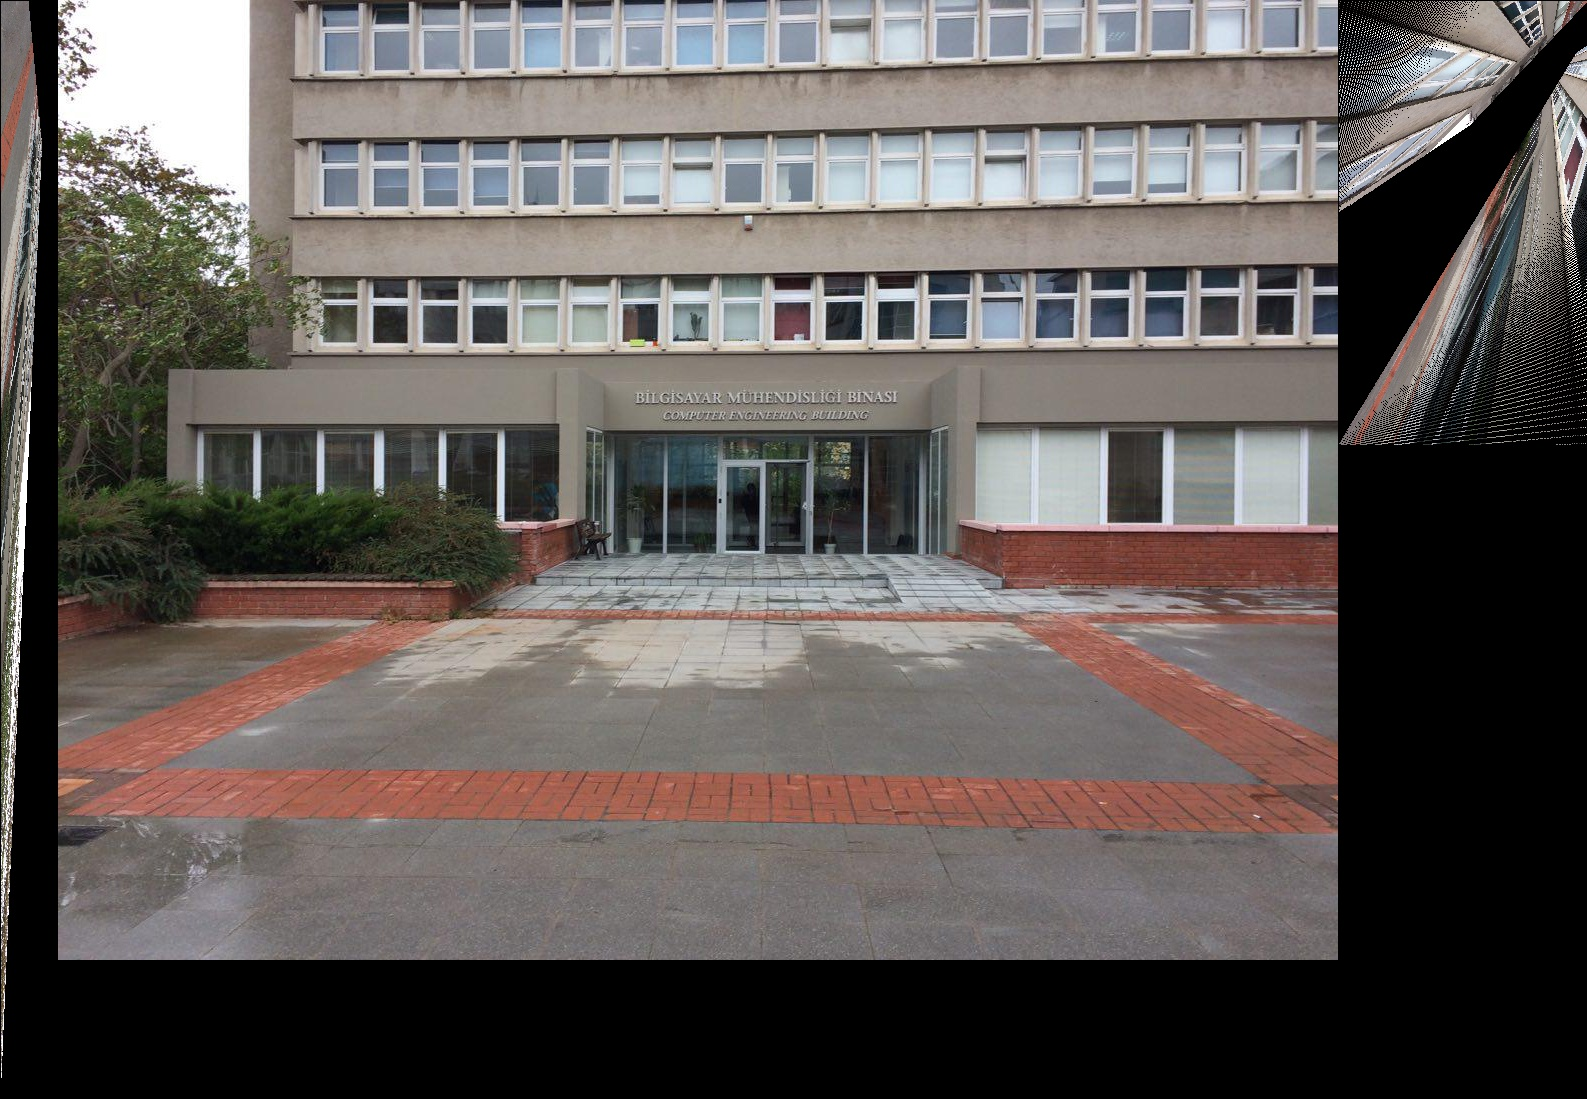
\includegraphics[width=1\columnwidth]{experiments/5points/final5wrong.jpg}
          \caption{
                \label{} Panoramic image
        }
        \centering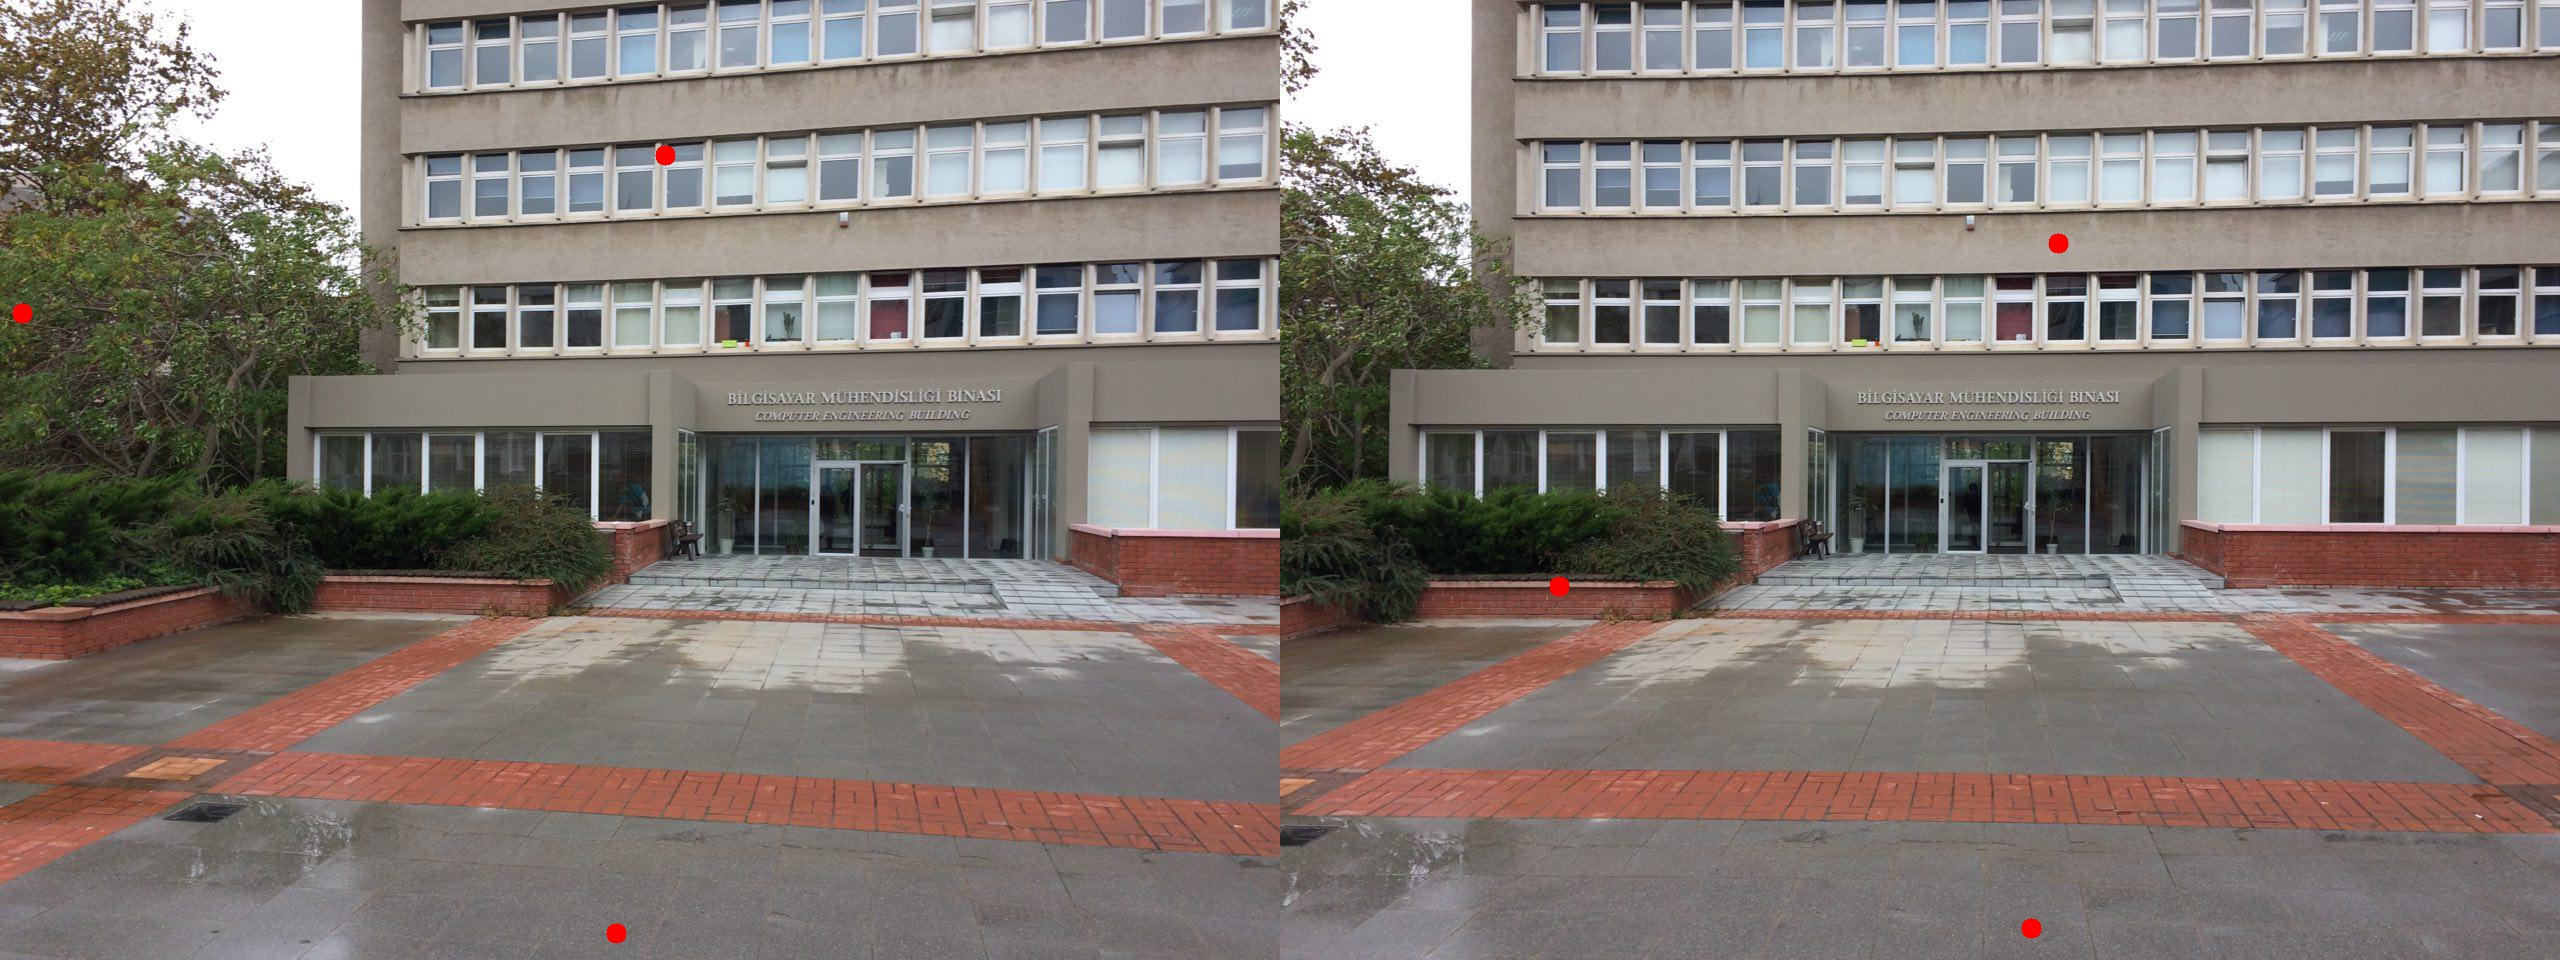
\includegraphics[width=1\columnwidth]{experiments/5points/left-1_middle5wrong.jpg}
          \caption{
                \label{} Common points between left and middle image.
        }
        \centering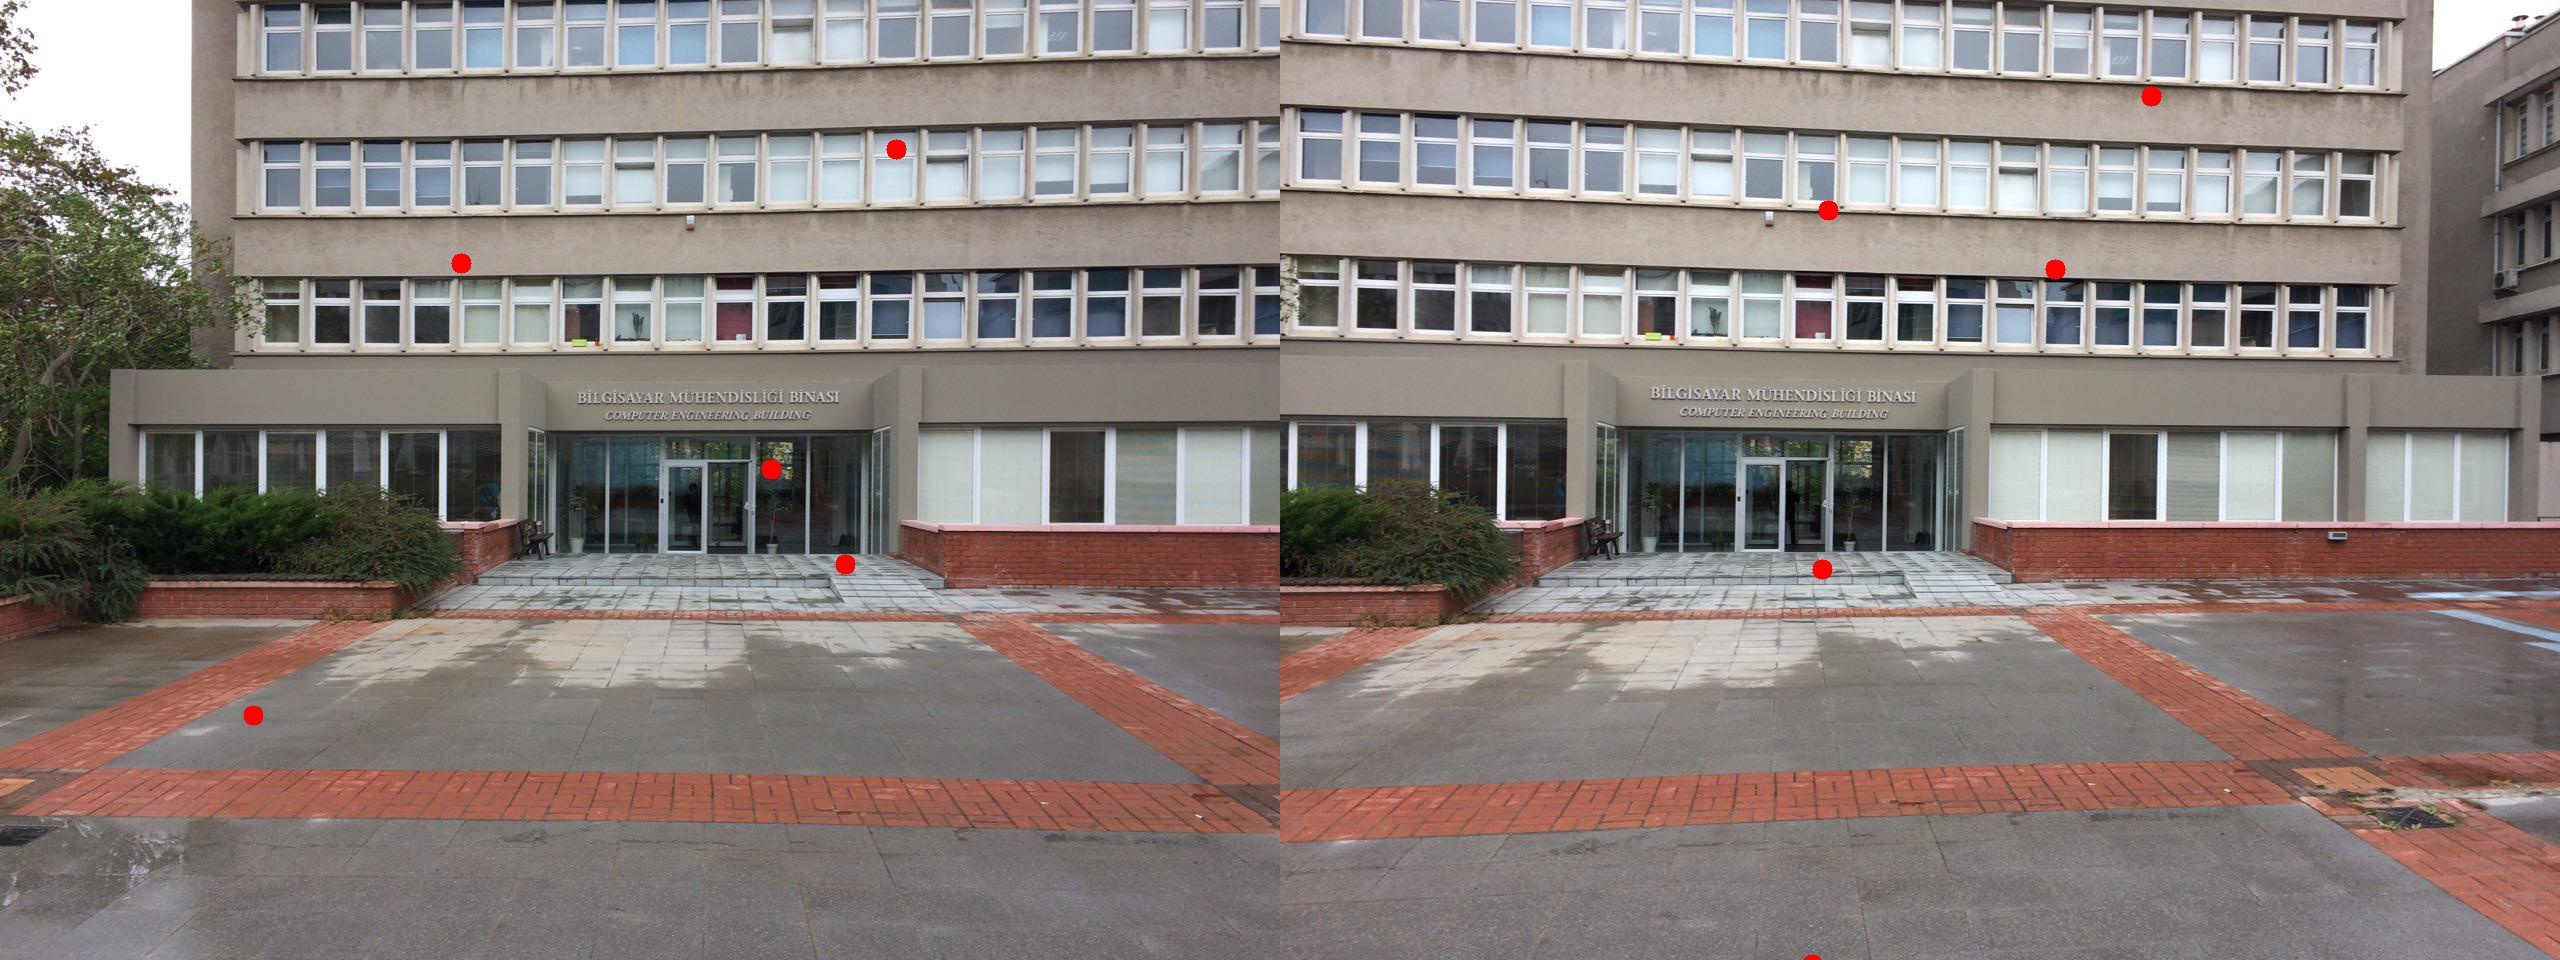
\includegraphics[width=1\columnwidth]{experiments/5points/middle_left-15wrong.jpg}
        \caption{
                \label{} Common points between middle and right image.
        }
\end{figure}
\FloatBarrier
\newpage
\subsubsection{5 Points with 5 Wrong Matches With Normalized Homography.}
\begin{figure}[!htb]
        \centering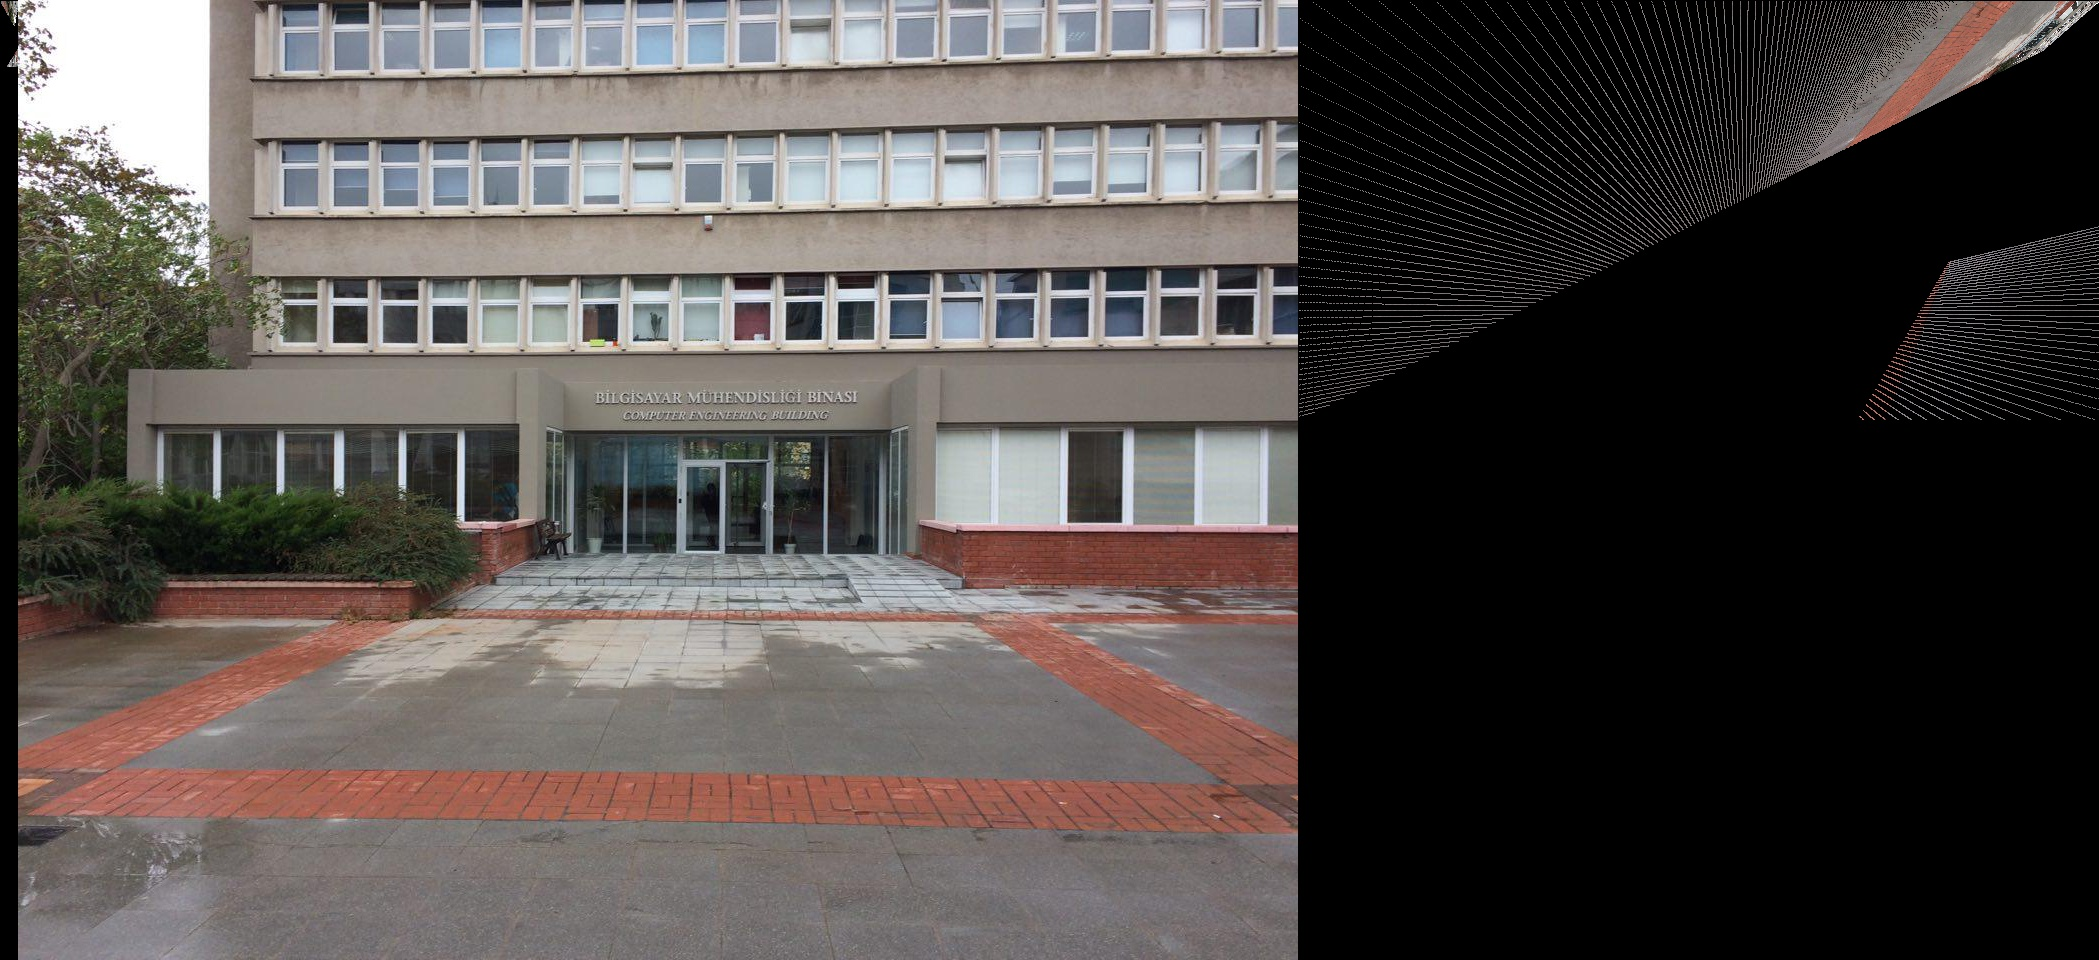
\includegraphics[width=1\columnwidth]{experiments/5points/norm/final5wrong.jpg}
          \caption{
                \label{} Panoramic image
        }
        \centering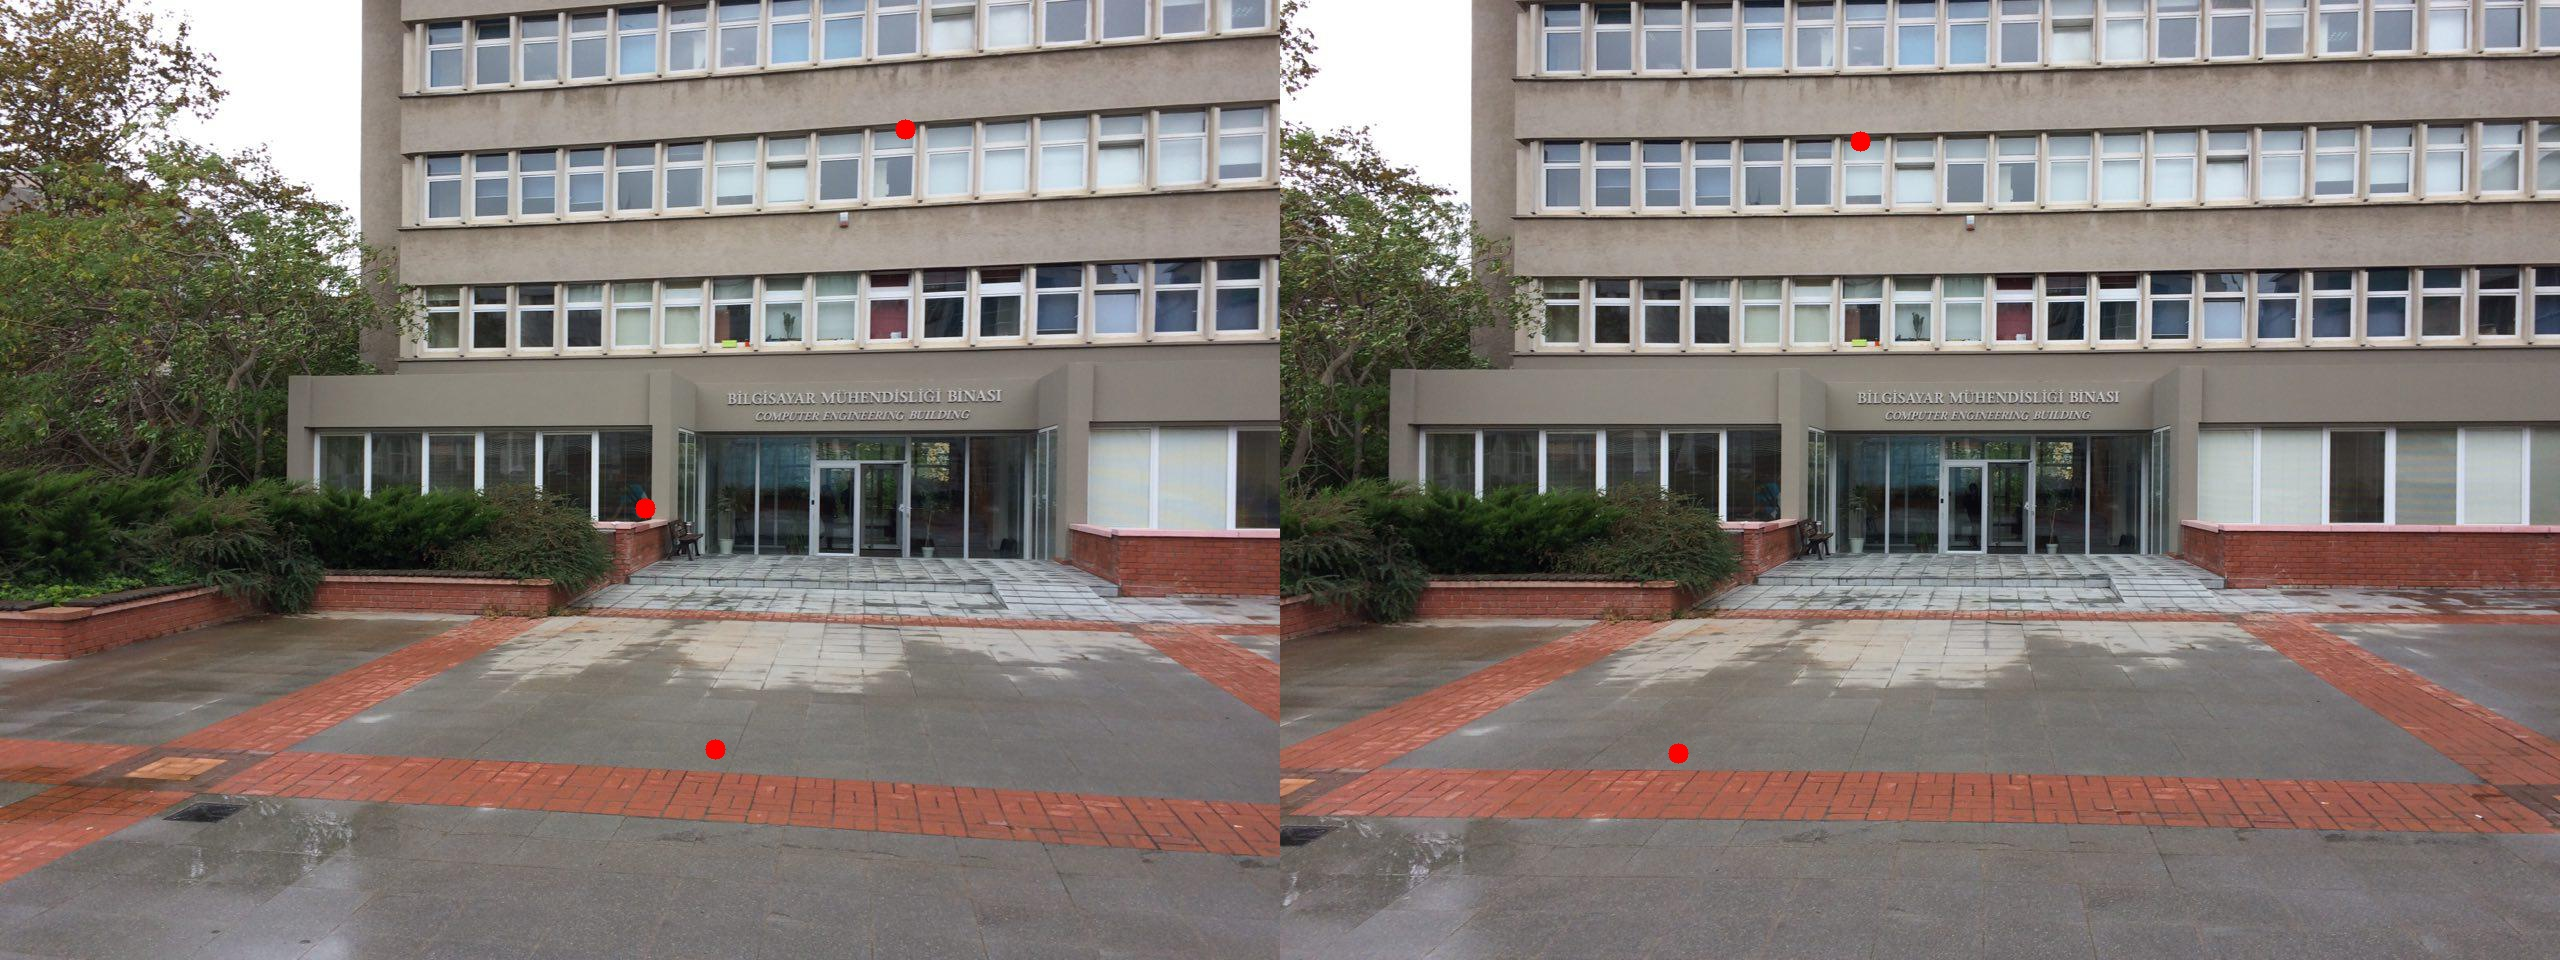
\includegraphics[width=1\columnwidth]{experiments/5points/norm/left-1_middle5wrong.jpg}
          \caption{
                \label{} Common points between left and middle image.
        }
        
        \centering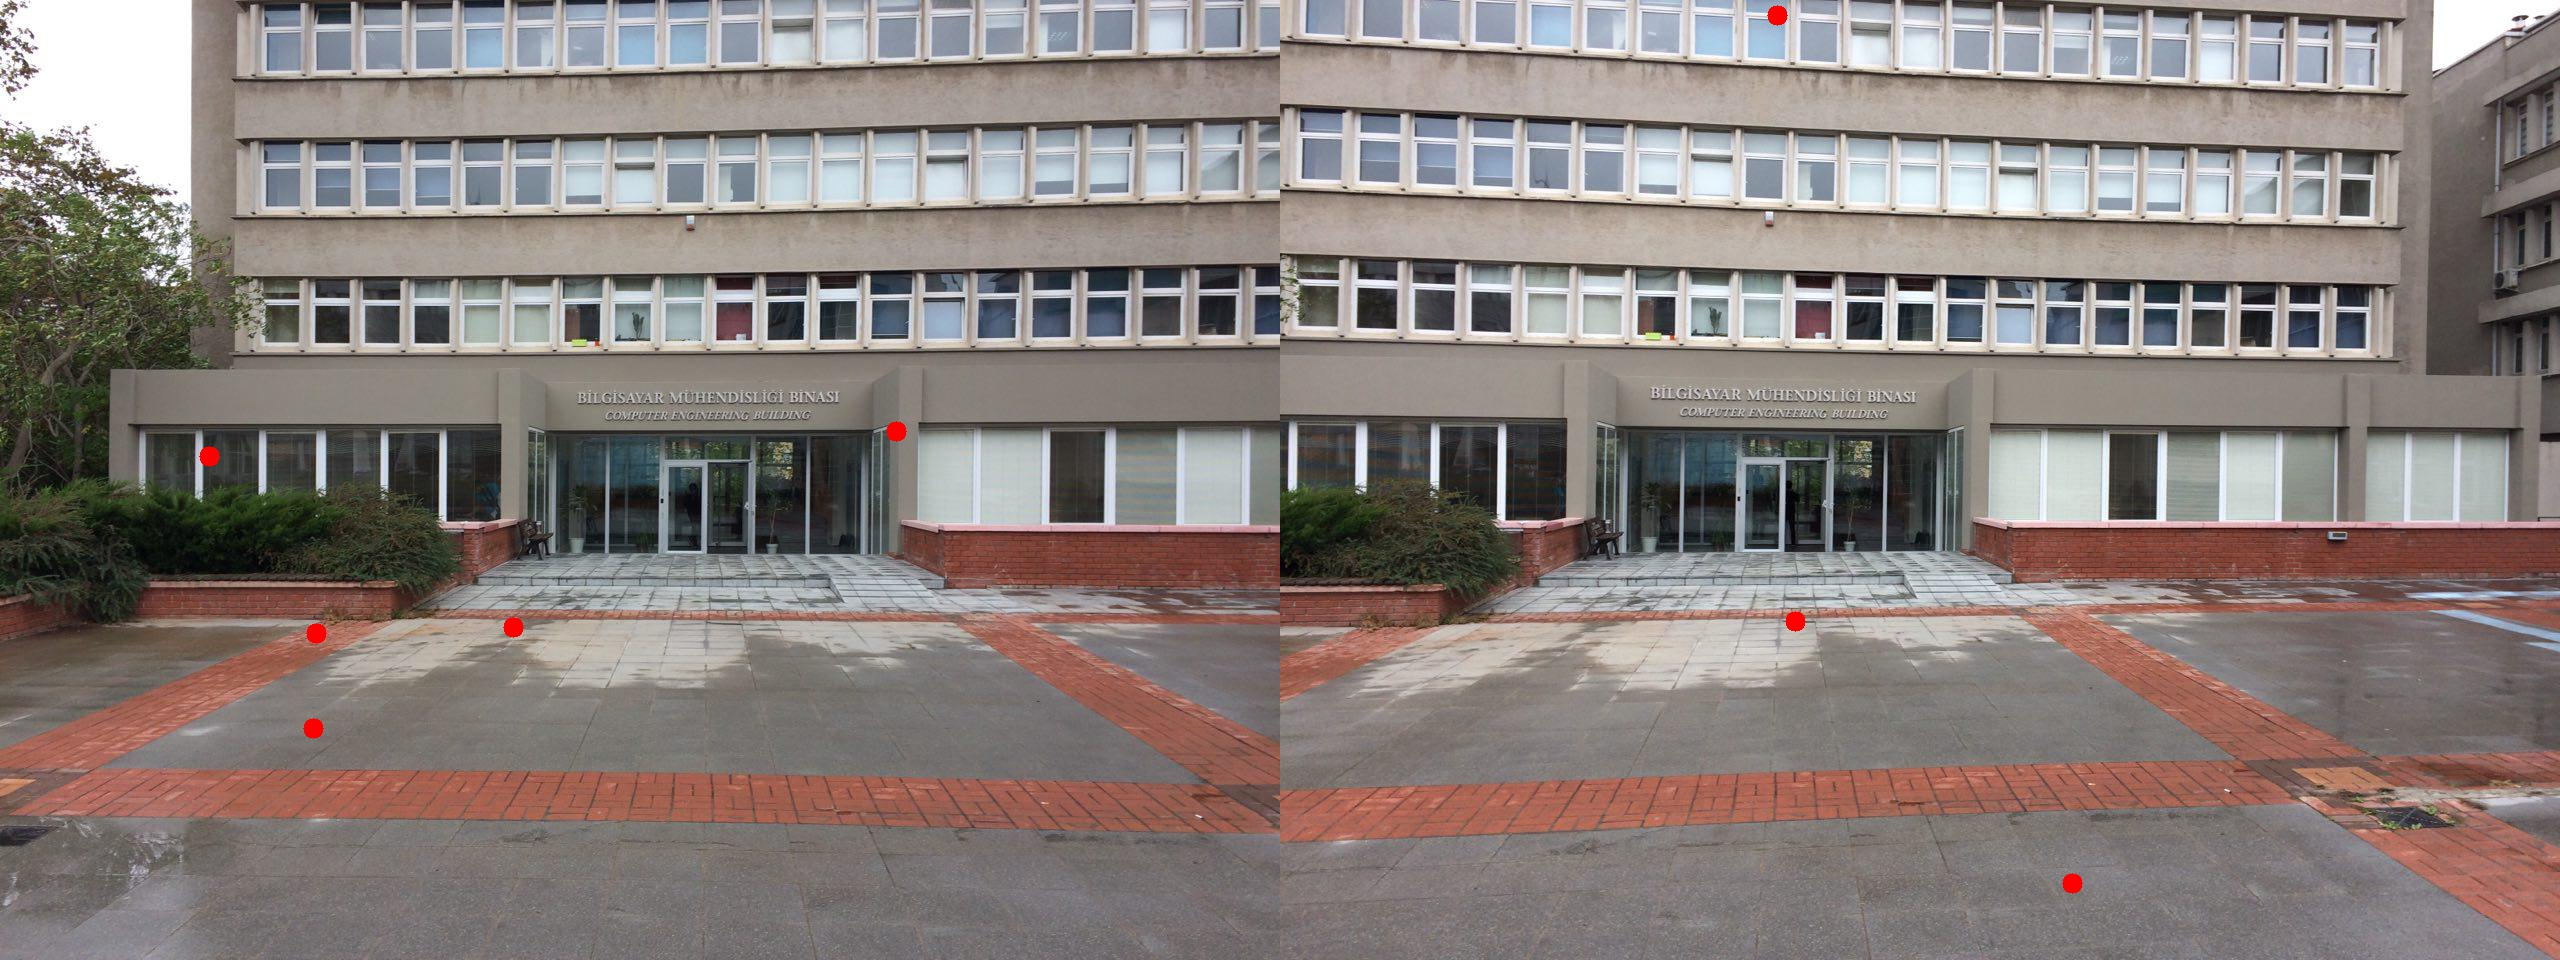
\includegraphics[width=1\columnwidth]{experiments/5points/norm/middle_left-15wrong.jpg}
        \caption{
                \label{} Common points between middle and right image.
        }
\end{figure}
\FloatBarrier
\newpage
\subsection{Experiments with 12 points}

\begin{figure}[!htb]
        \centering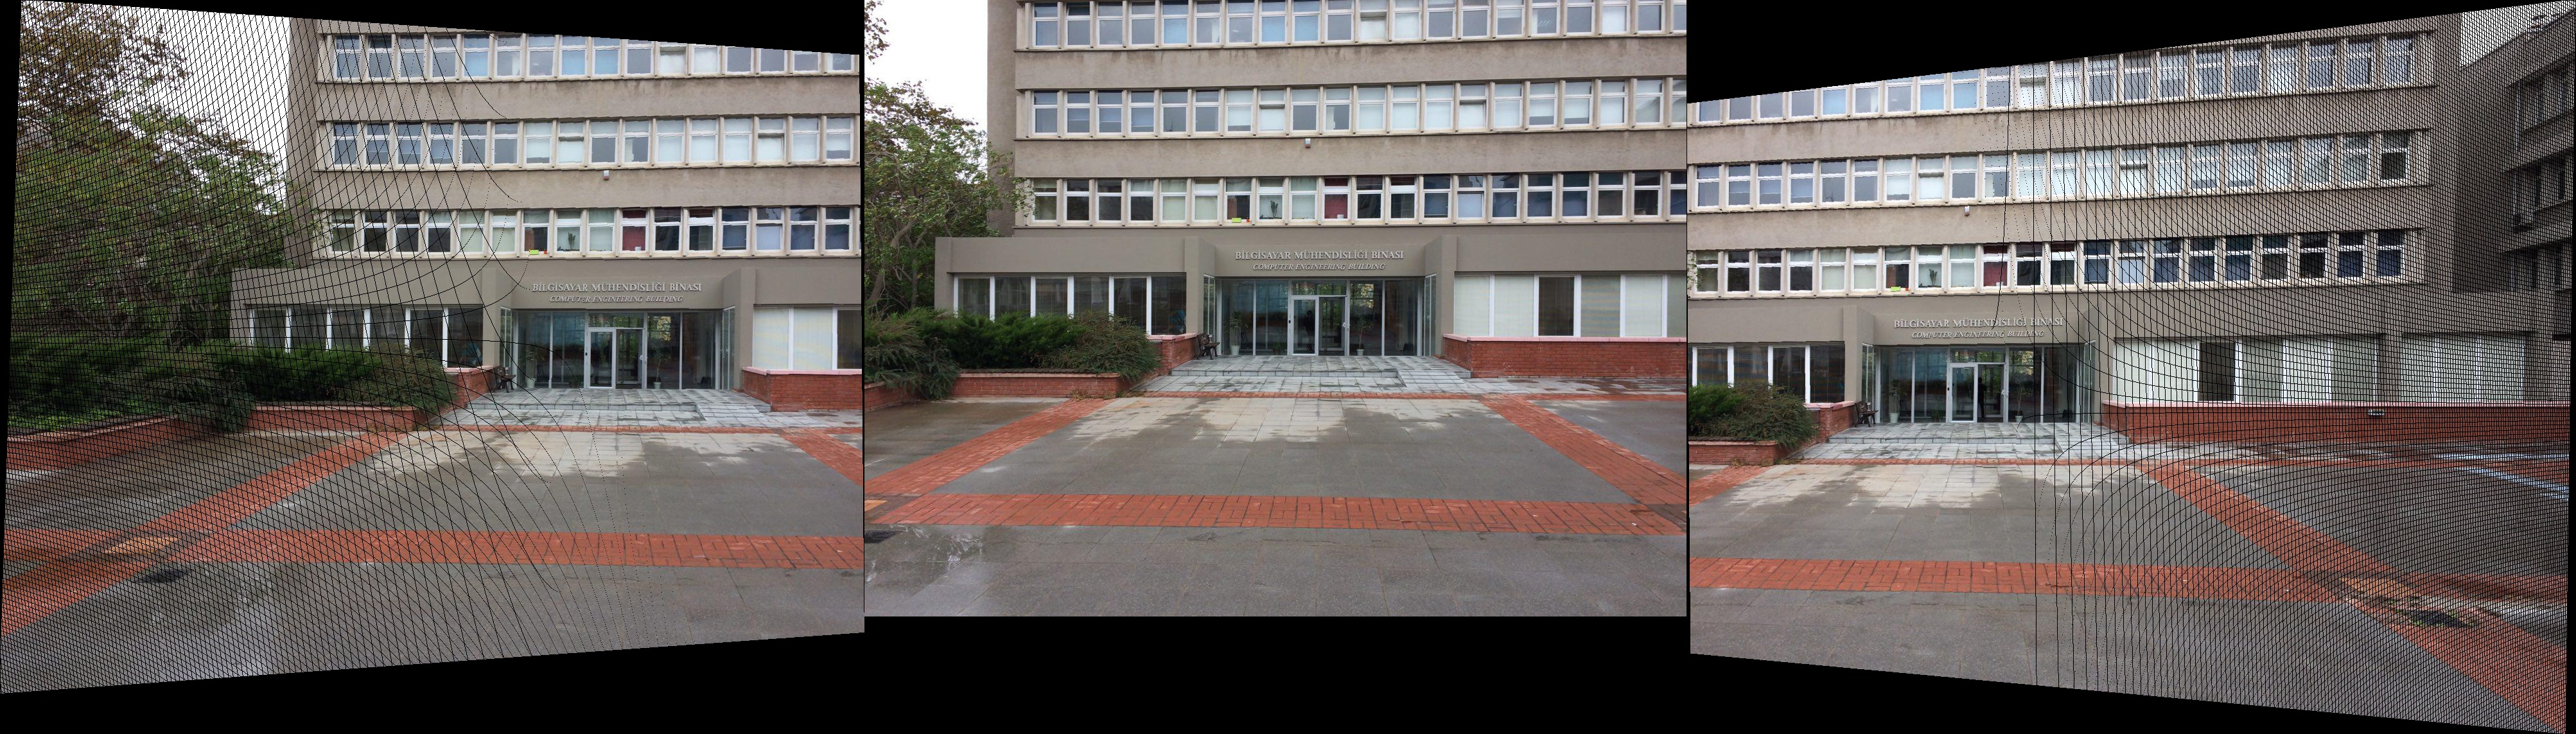
\includegraphics[width=1\columnwidth]{experiments/12points/finalNonewrong.jpg}
          \caption{
                \label{} Panoramic image
        }
        \centering\includegraphics[width=1\columnwidth]{experiments/12points/left-1_middleNonewrong.jpg}
          \caption{
                \label{} Common points between left and middle image.
        }
        \centering\includegraphics[width=1\columnwidth]{experiments/12points/middle_left-1Nonewrong.jpg}
        \caption{
                \label{} Common points between middle and right image.
        }
\end{figure}
\FloatBarrier
\newpage
\subsubsection{12 Points With Normalized Homography}
\begin{figure}[!htb]
        \centering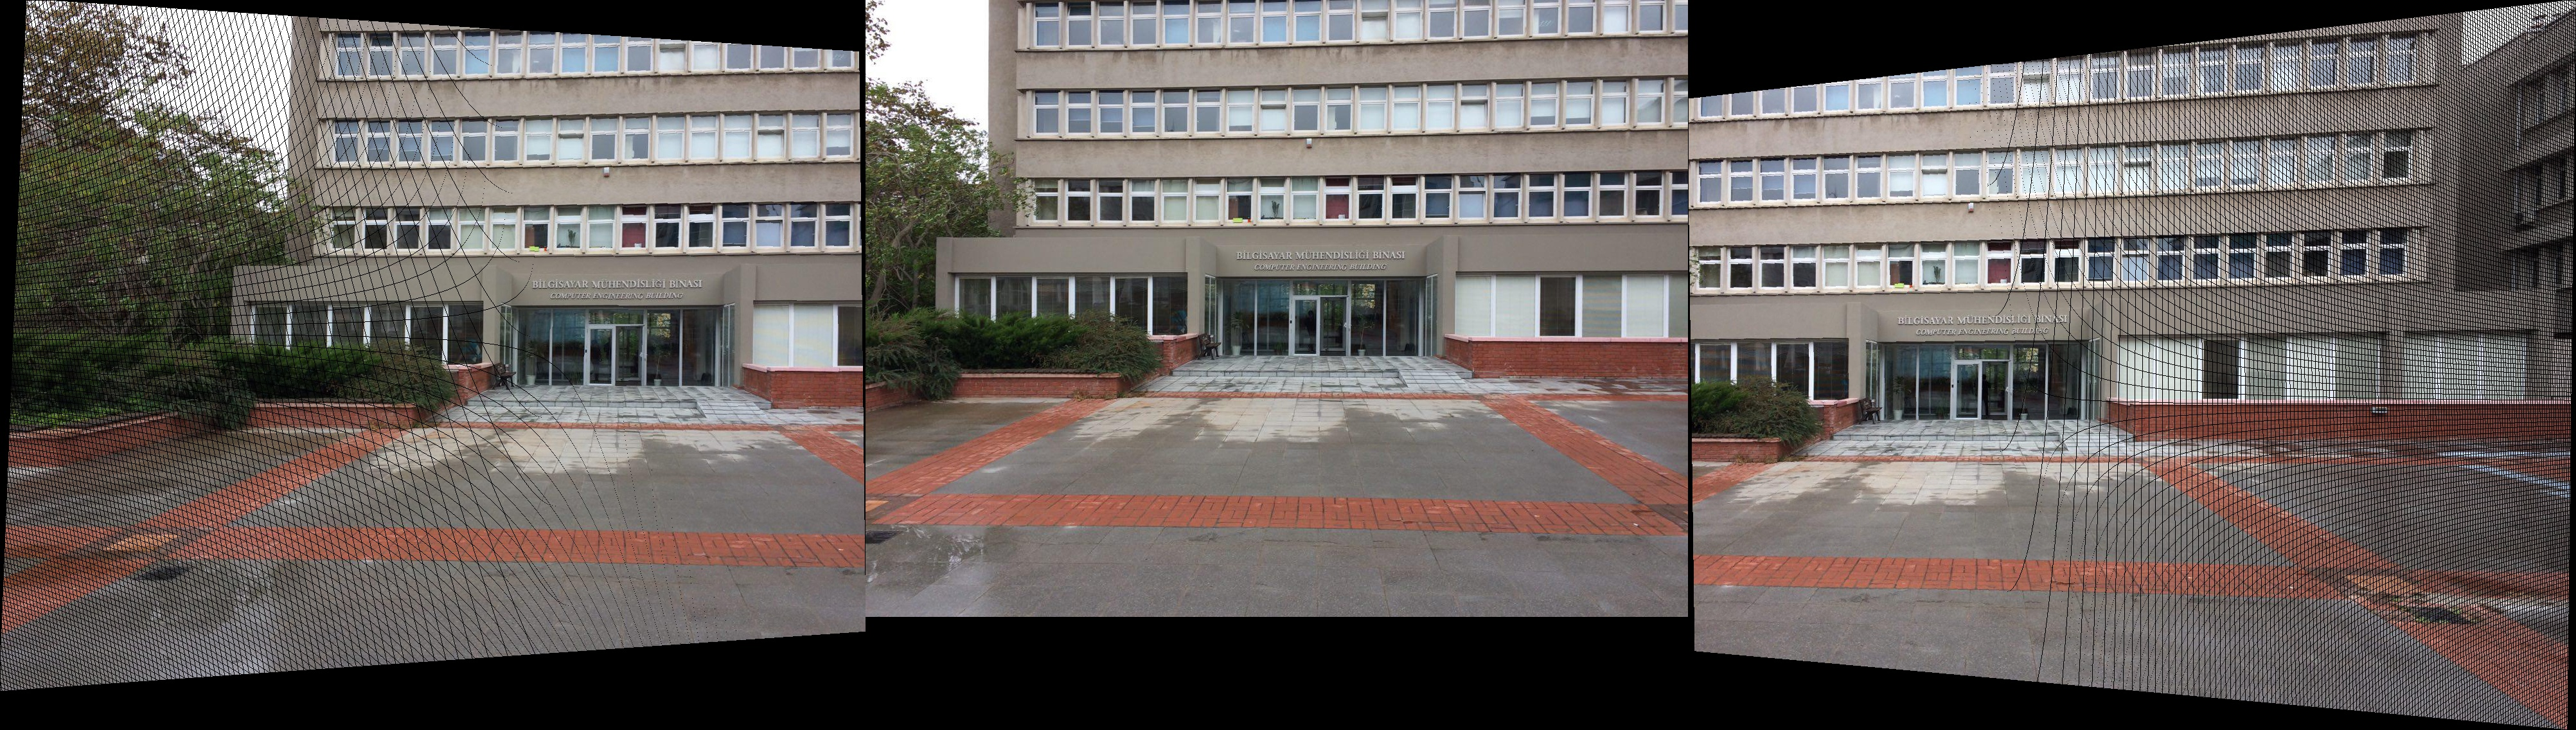
\includegraphics[width=1\columnwidth]{experiments/12points/norm/finalNonewrong.jpg}
          \caption{
                \label{} Panoramic image
        }
        \centering\includegraphics[width=1\columnwidth]{experiments/12points/norm/left-1_middleNonewrong.jpg}
          \caption{
                \label{} Common points between left and middle image.
        }
        \centering\includegraphics[width=1\columnwidth]{experiments/12points/norm/middle_left-1Nonewrong.jpg}
        \caption{
                \label{} Common points between middle and right image.
        }
\end{figure}

\FloatBarrier

\newpage
\subsubsection{12 Points with 3 Wrong Matches Without Normalized Homography.}

\begin{figure}[!htb]
        \centering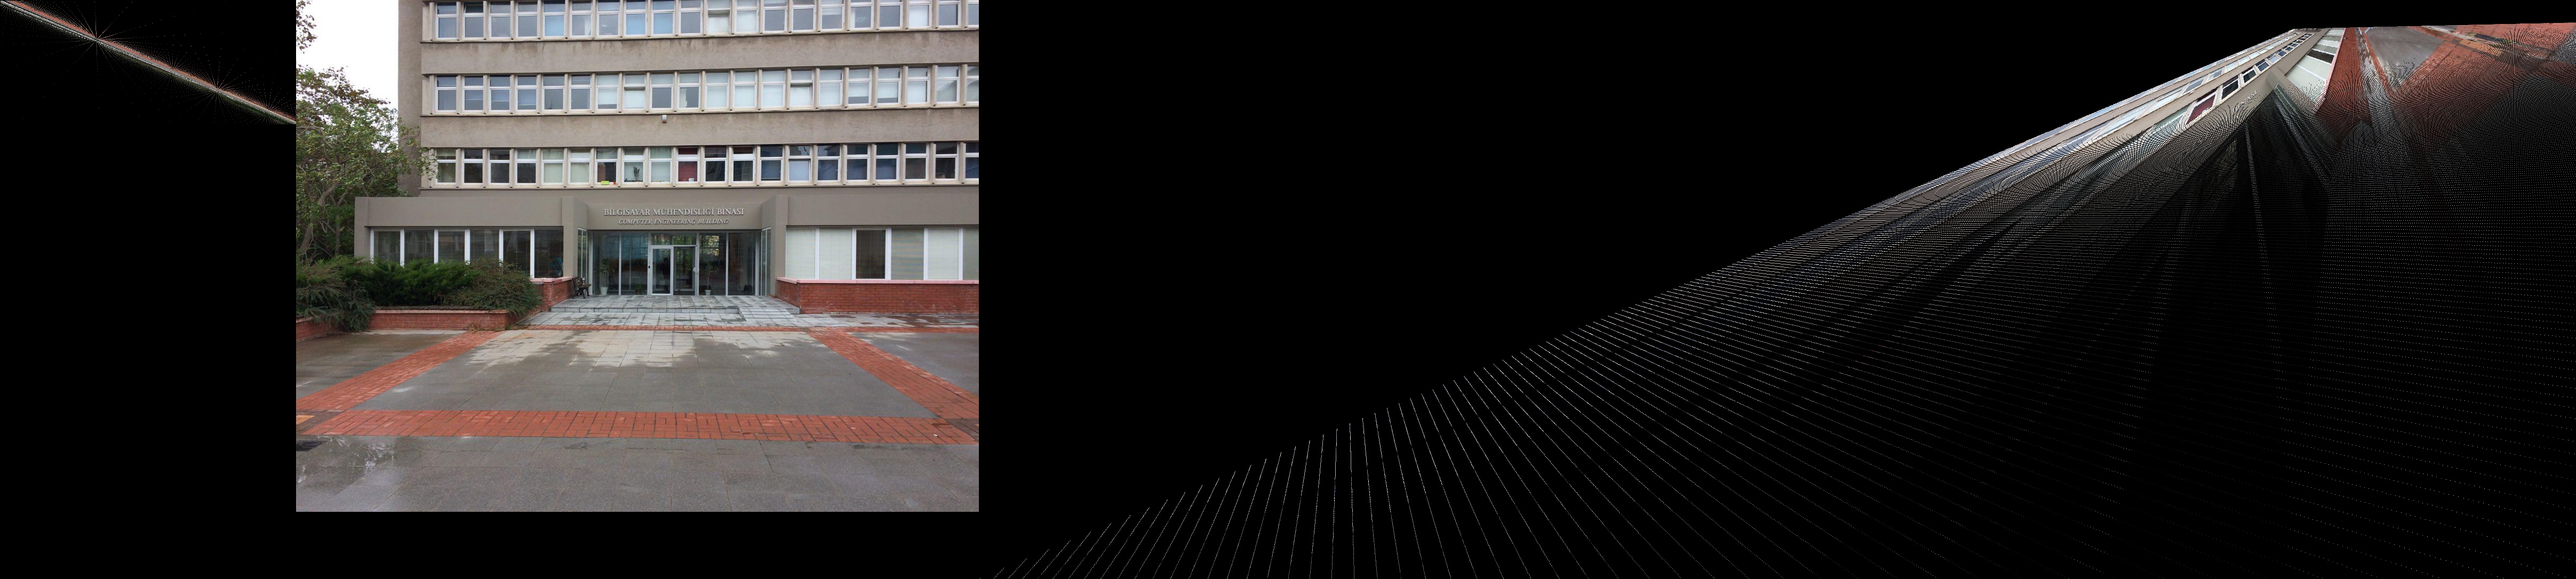
\includegraphics[width=1\columnwidth]{experiments/12points/final3wrong.jpg}
          \caption{
                \label{} Panoramic image
        }
        \centering\includegraphics[width=1\columnwidth]{experiments/12points/left-1_middle3wrong.jpg}
          \caption{
                \label{} Common points between left and middle image.
        }
        \centering\includegraphics[width=1\columnwidth]{experiments/12points/middle_left-13wrong.jpg}
        \caption{
                \label{} Common points between middle and right image.
        }
\end{figure}
\FloatBarrier
\newpage
\subsubsection{12 Points with 3 Wrong Matches With Normalized Homography.}
\begin{figure}[!htb]
        \centering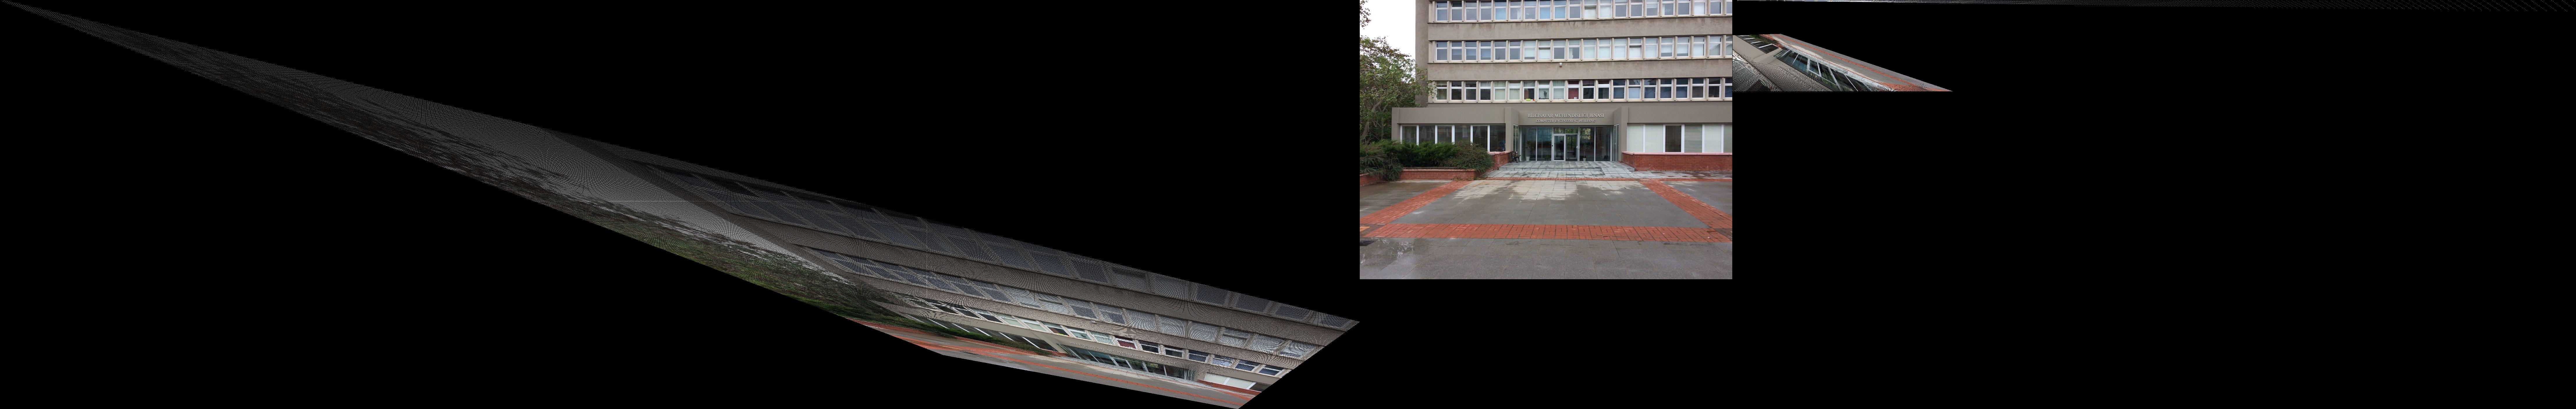
\includegraphics[width=1\columnwidth]{experiments/12points/norm/final3wrong.jpg}
          \caption{
                \label{} Panoramic image
        }
        \centering\includegraphics[width=1\columnwidth]{experiments/12points/norm/left-1_middle3wrong.jpg}
          \caption{
                \label{} Common points between left and middle image.
        }
        \centering\includegraphics[width=1\columnwidth]{experiments/12points/norm/middle_left-13wrong.jpg}
        \caption{
                \label{} Common points between middle and right image.
        }
\end{figure}
\FloatBarrier
\newpage
\subsubsection{12 Points with 5 Wrong Matches Without Normalized Homography.}
\begin{figure}[!htb]
        \centering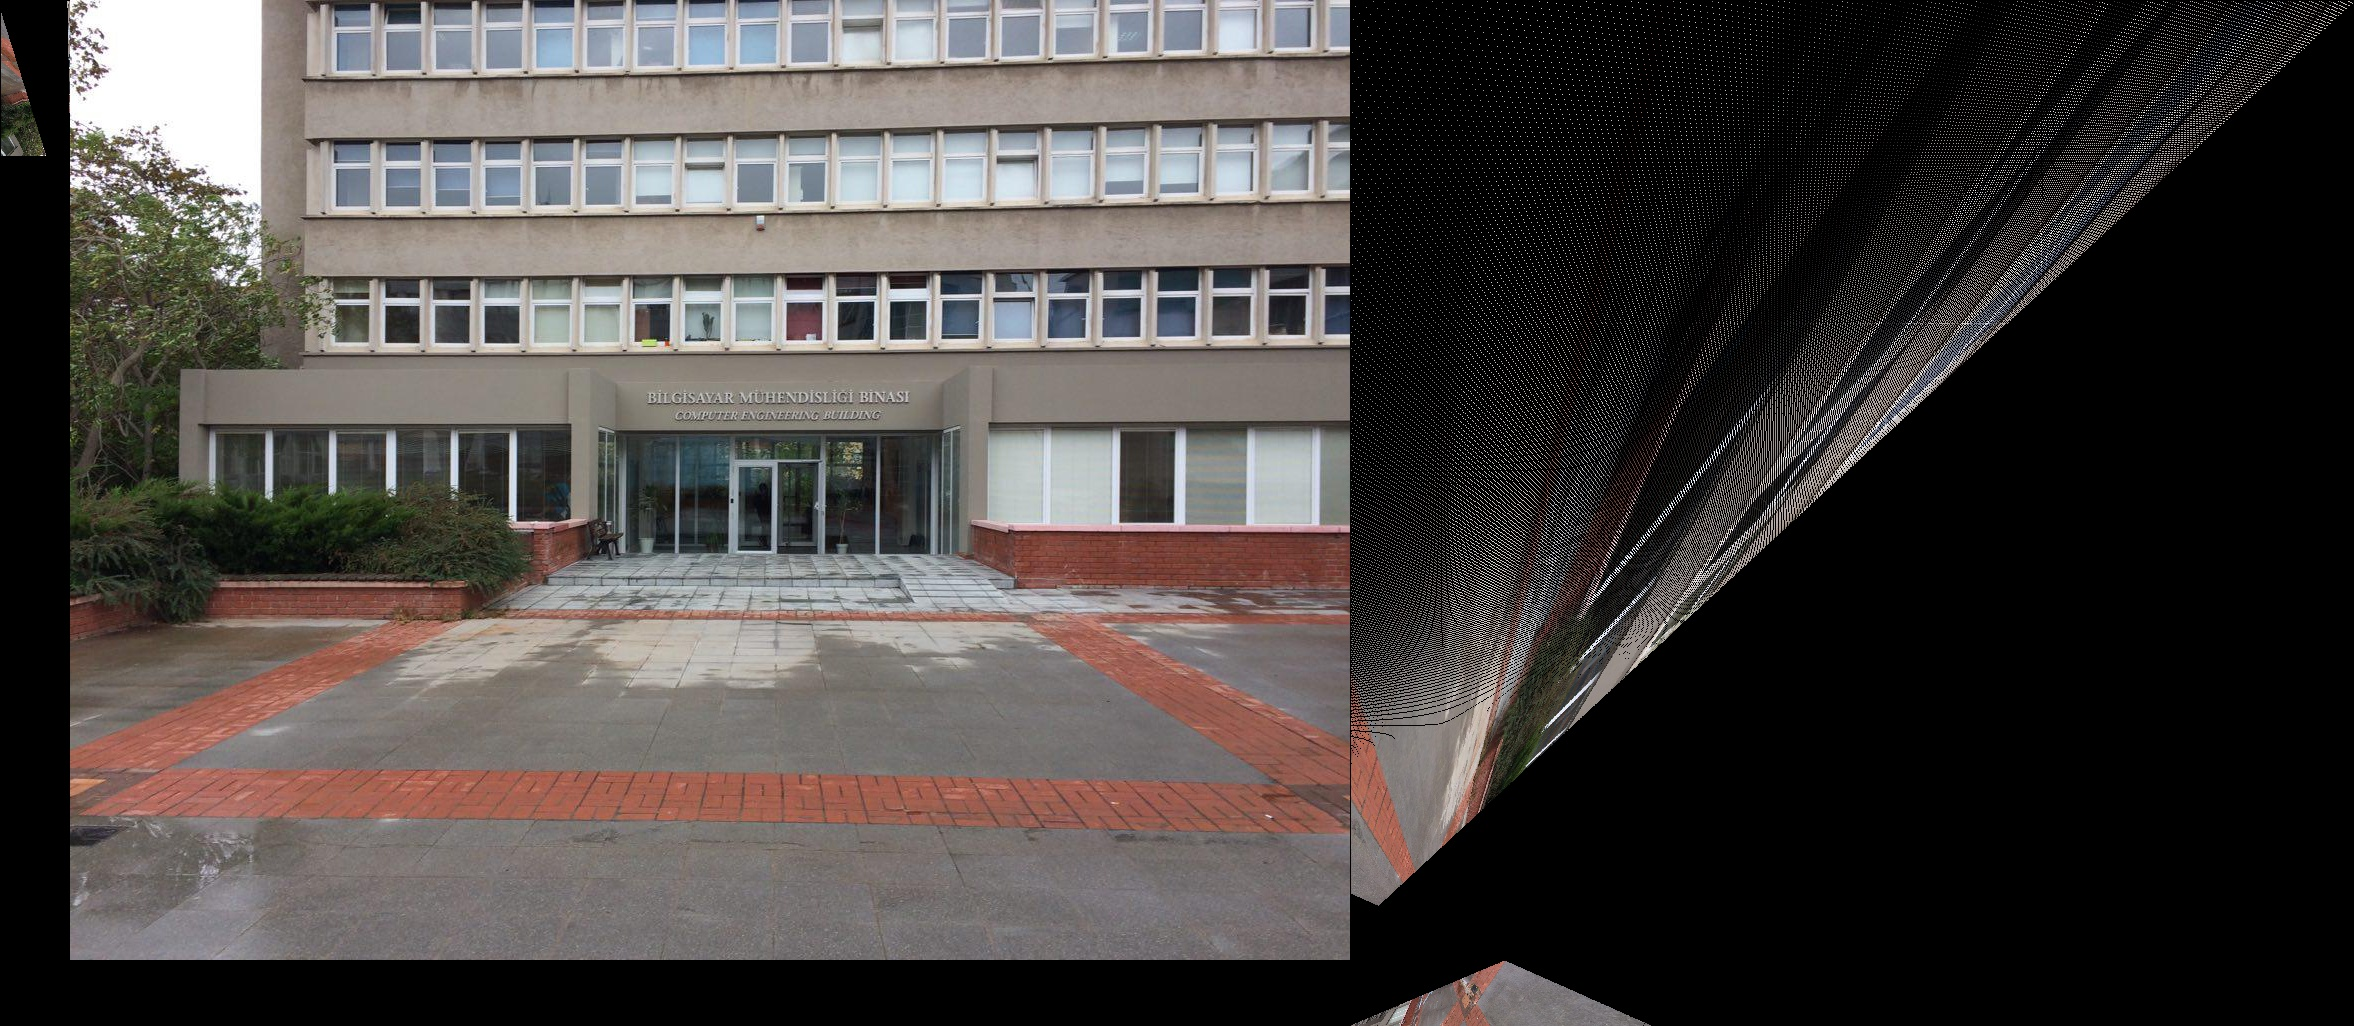
\includegraphics[width=1\columnwidth]{experiments/12points/final5wrong.jpg}
          \caption{
                \label{} Panoramic image
        }
        \centering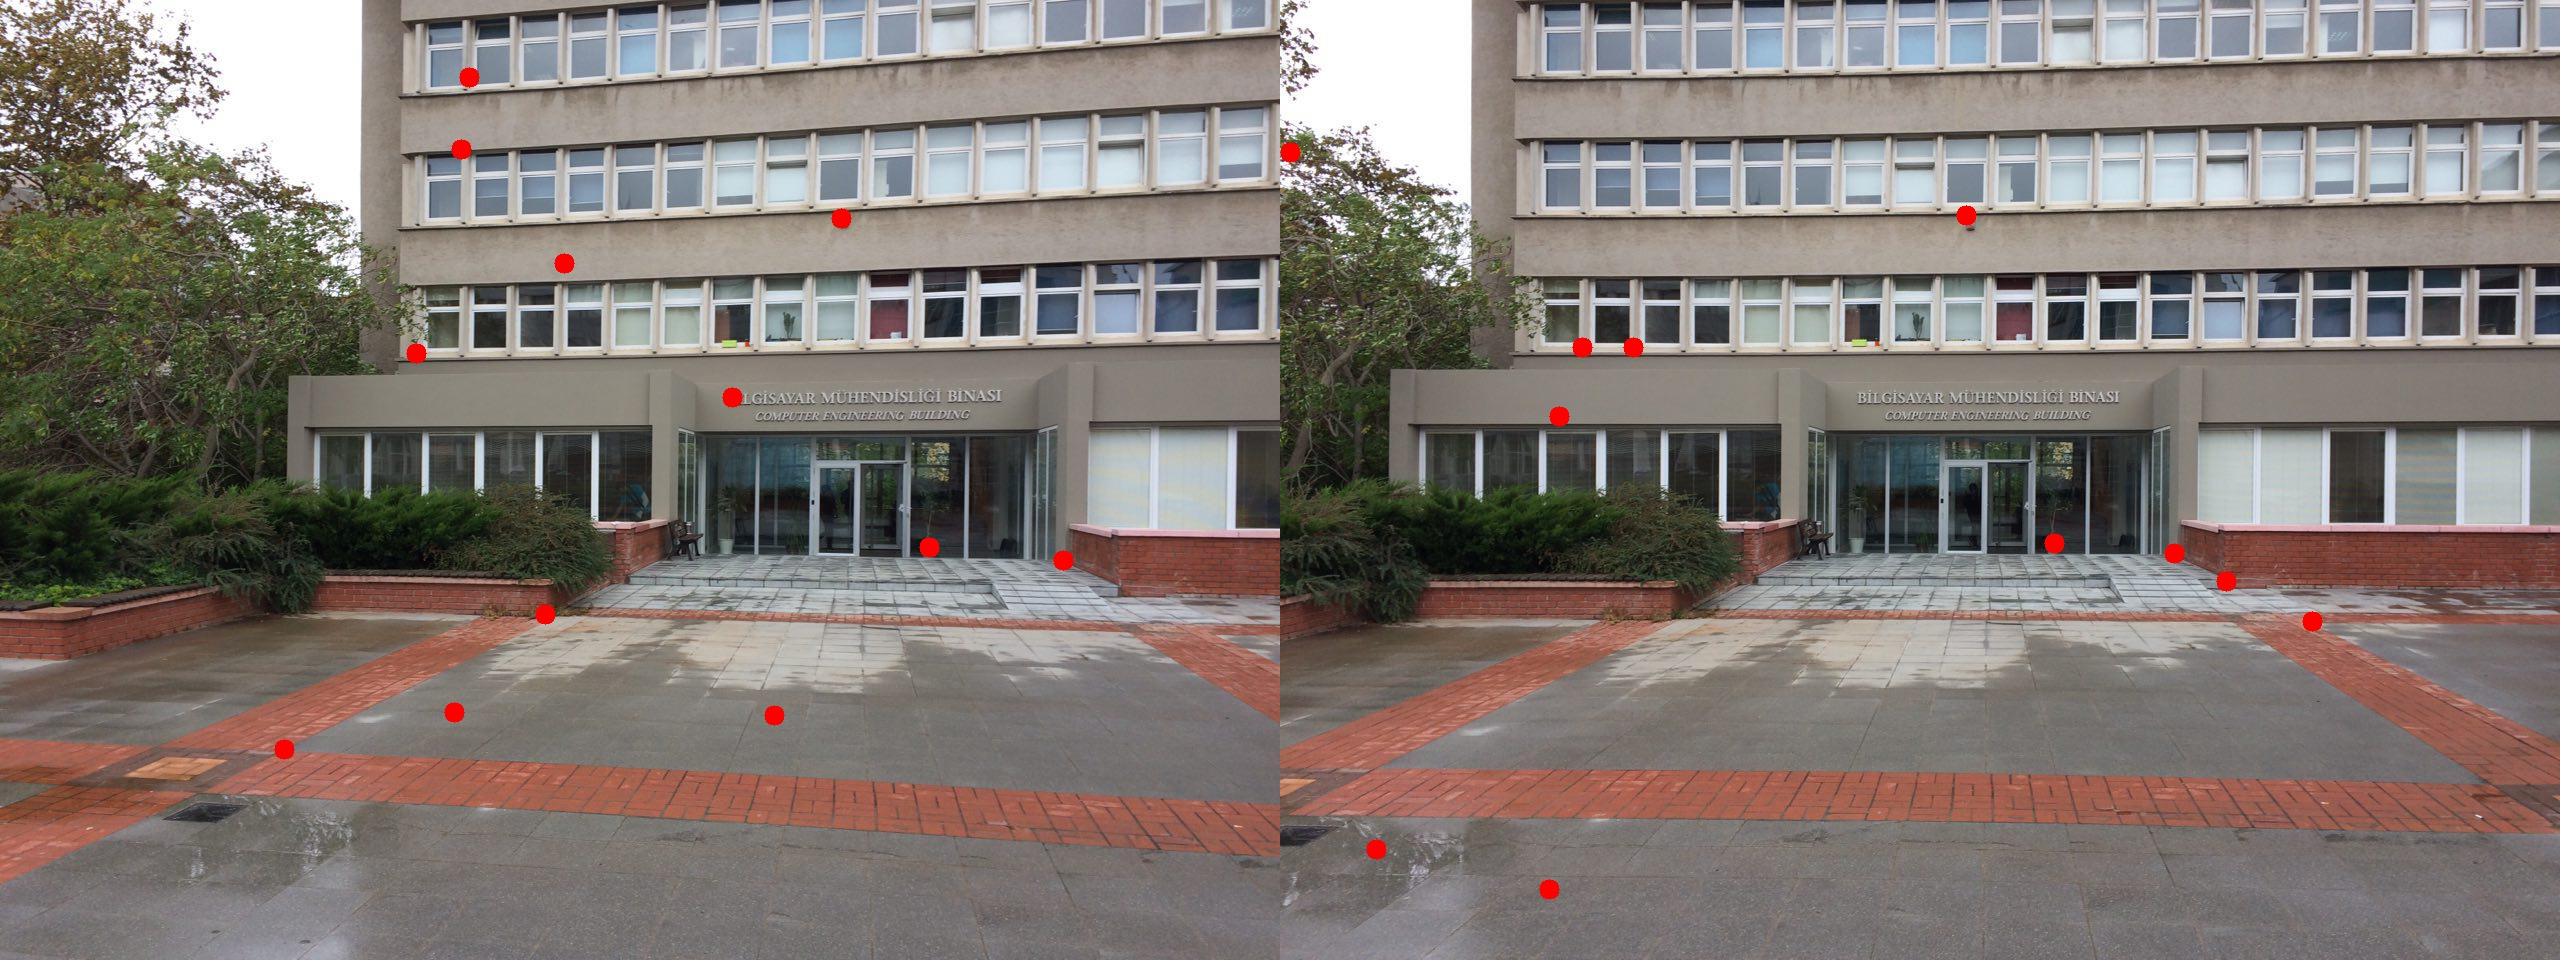
\includegraphics[width=1\columnwidth]{experiments/12points/left-1_middle5wrong.jpg}
          \caption{
                \label{} Common points between left and middle image.
        }
        \centering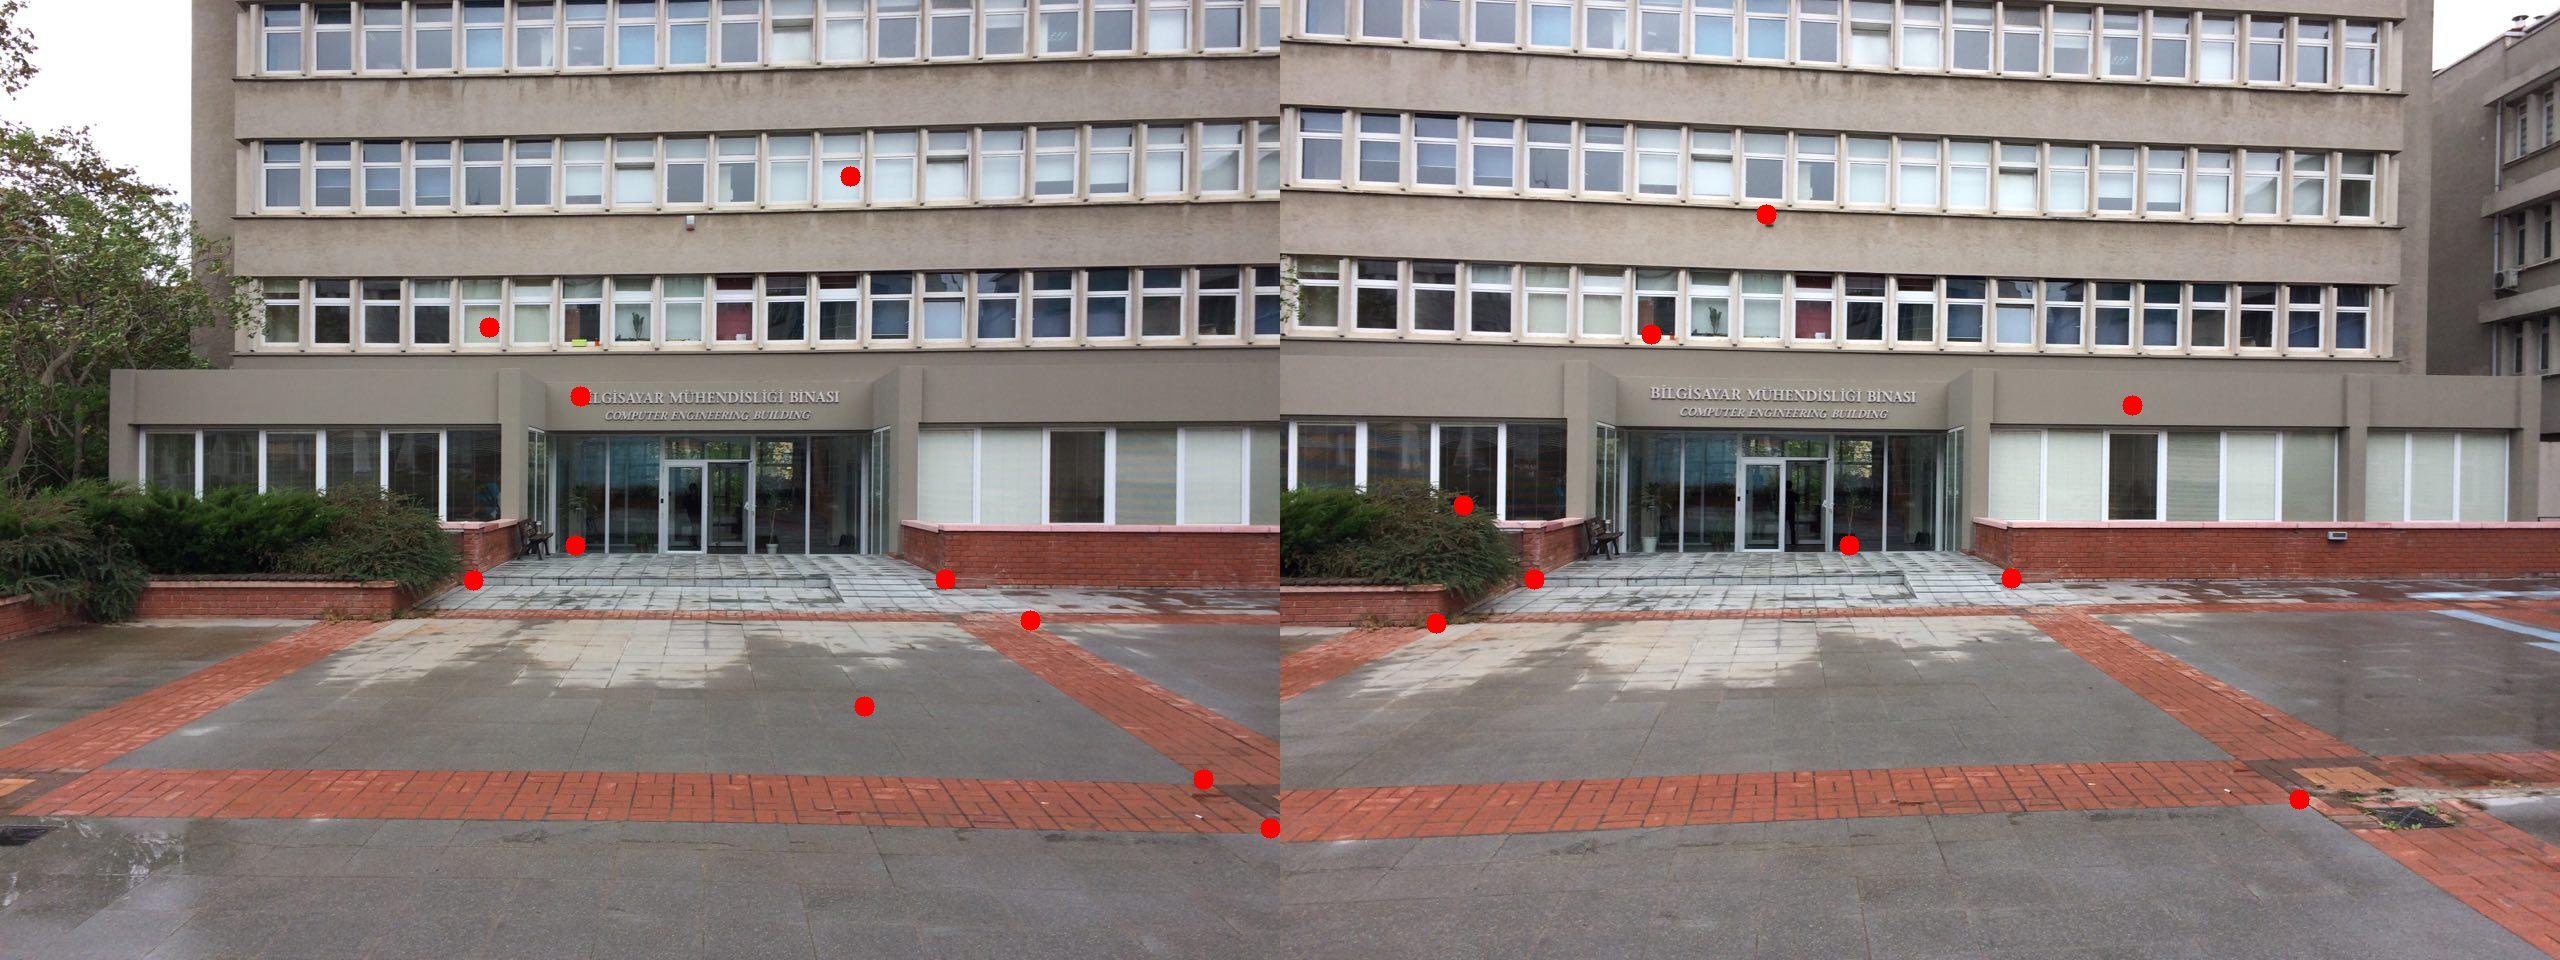
\includegraphics[width=1\columnwidth]{experiments/12points/middle_left-15wrong.jpg}
        \caption{
                \label{} Common points between middle and right image.
        }
\end{figure}
\FloatBarrier
\newpage
\subsubsection{12 Points with 5 Wrong Matches With Normalized Homography.}
\begin{figure}[!htb]
        \centering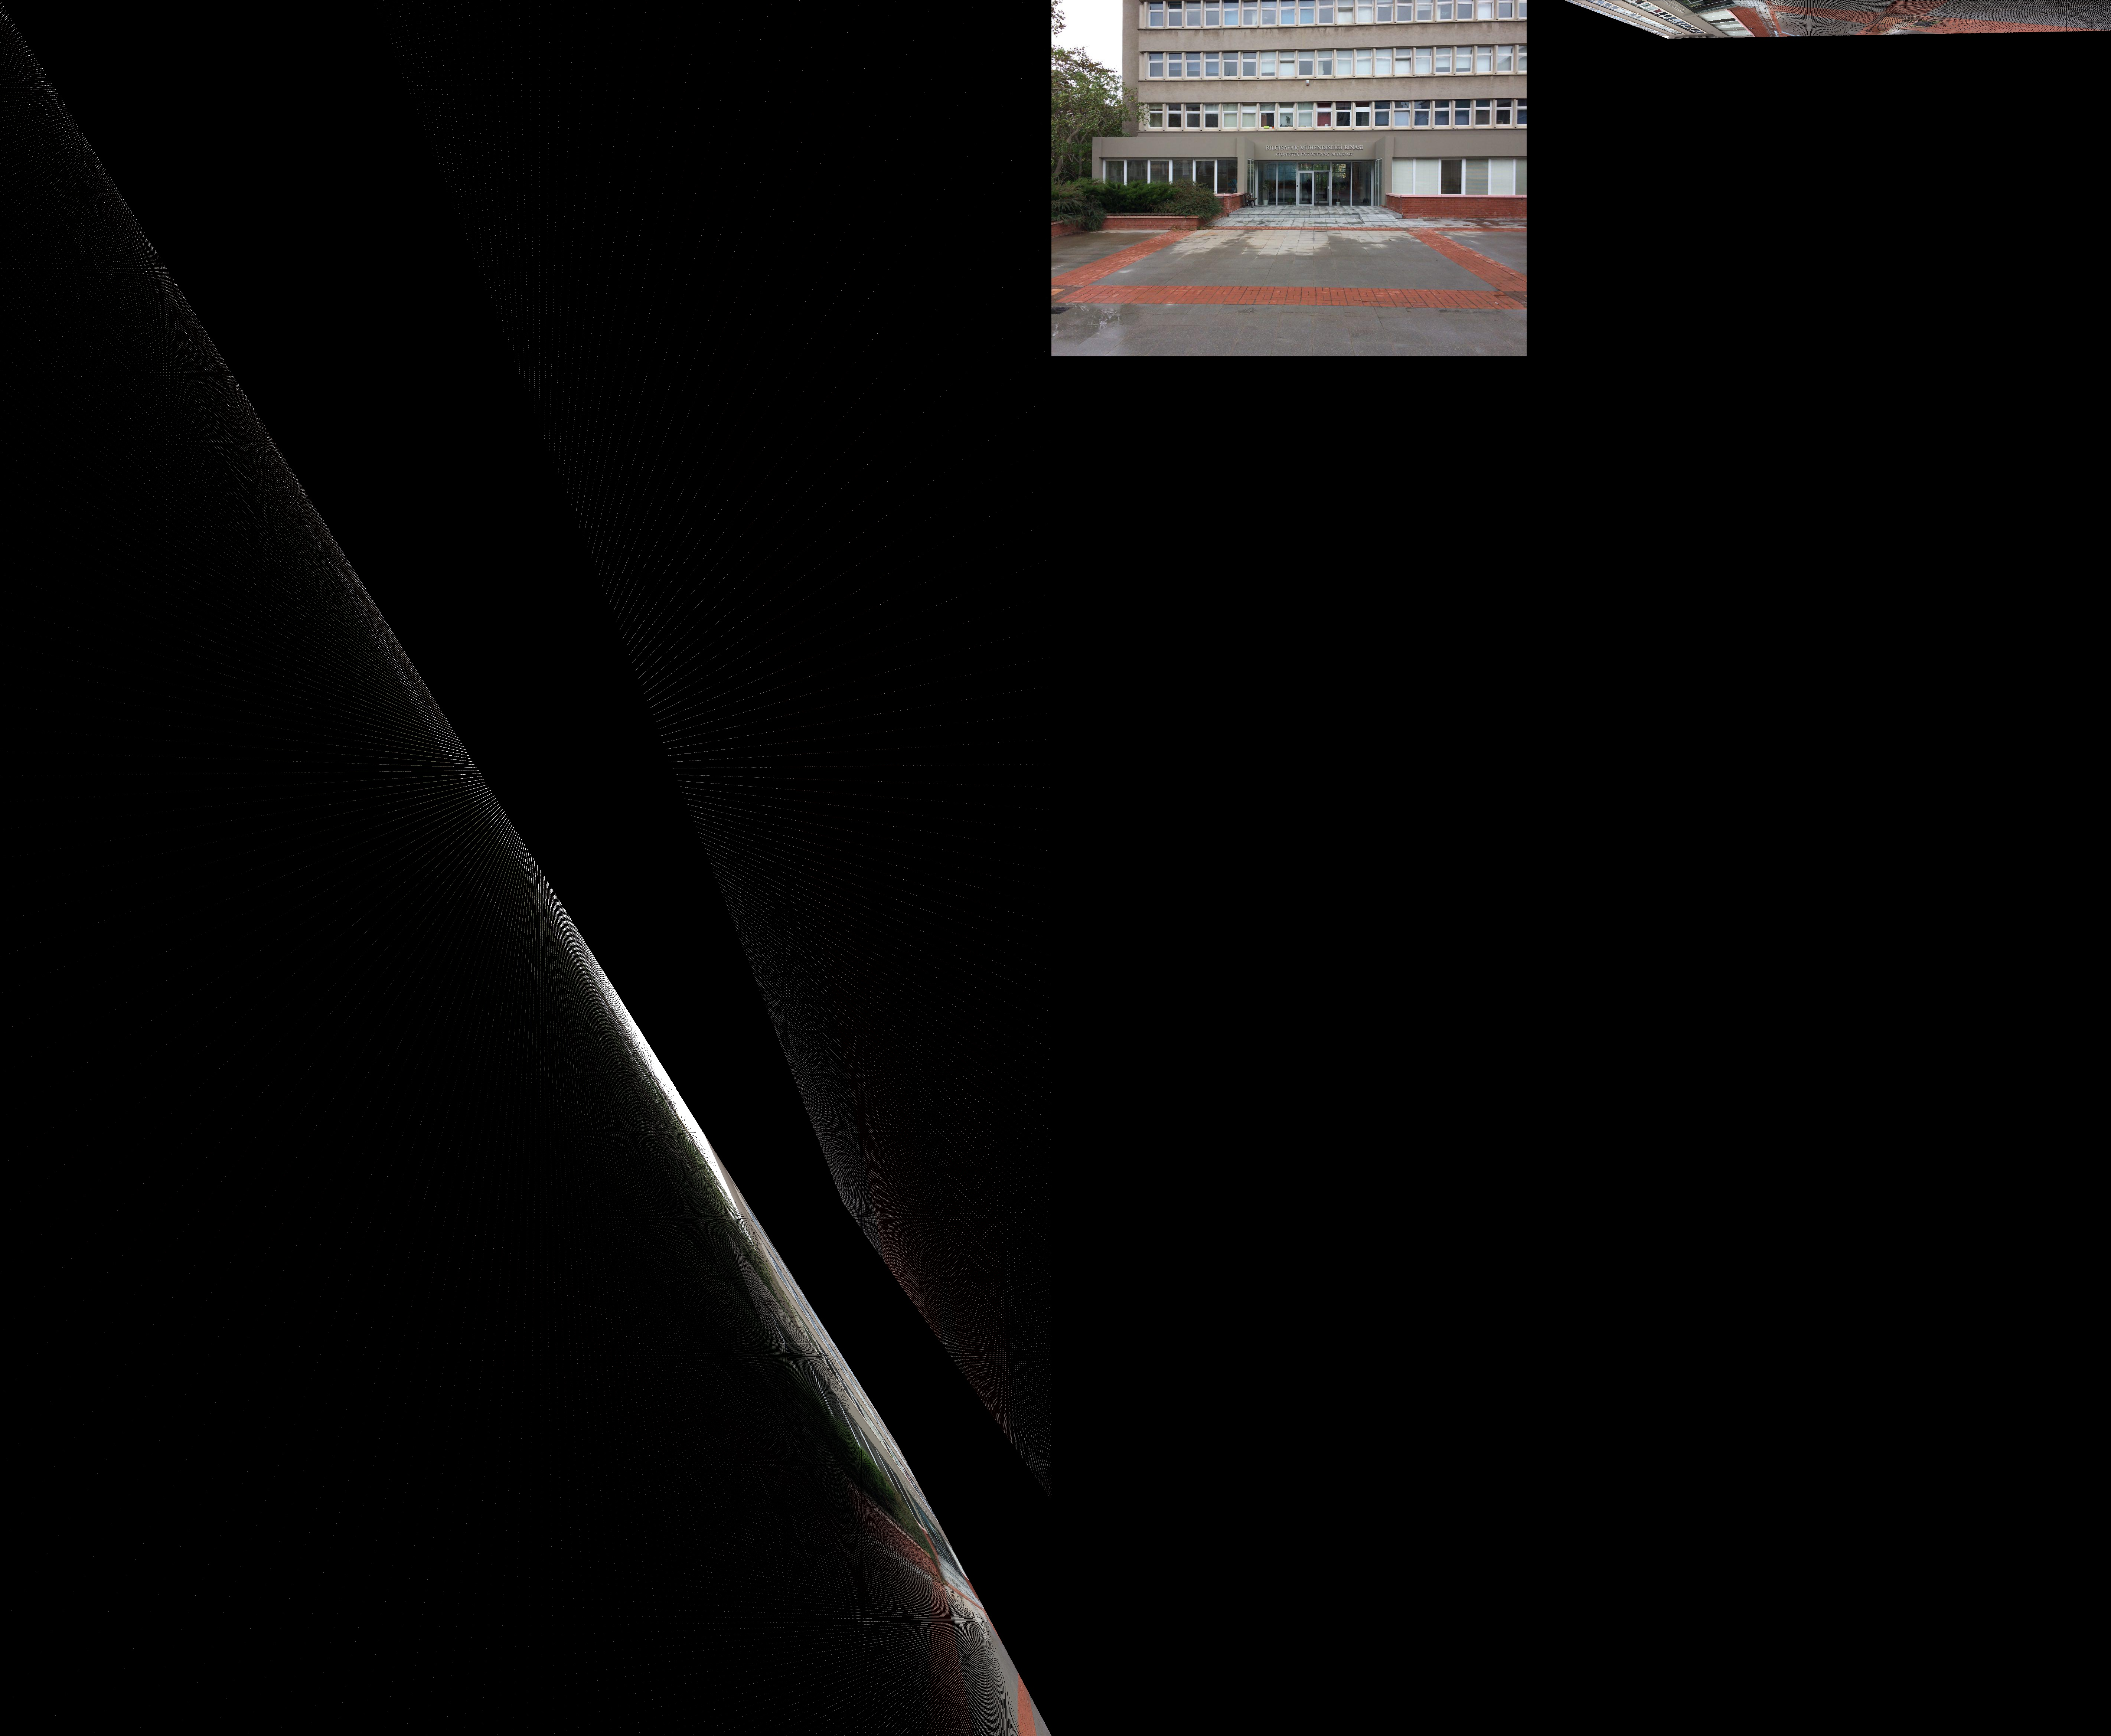
\includegraphics[width=1\columnwidth]{experiments/12points/norm/final5wrong.jpg}
          \caption{
                \label{} Panoramic image
        }
        \centering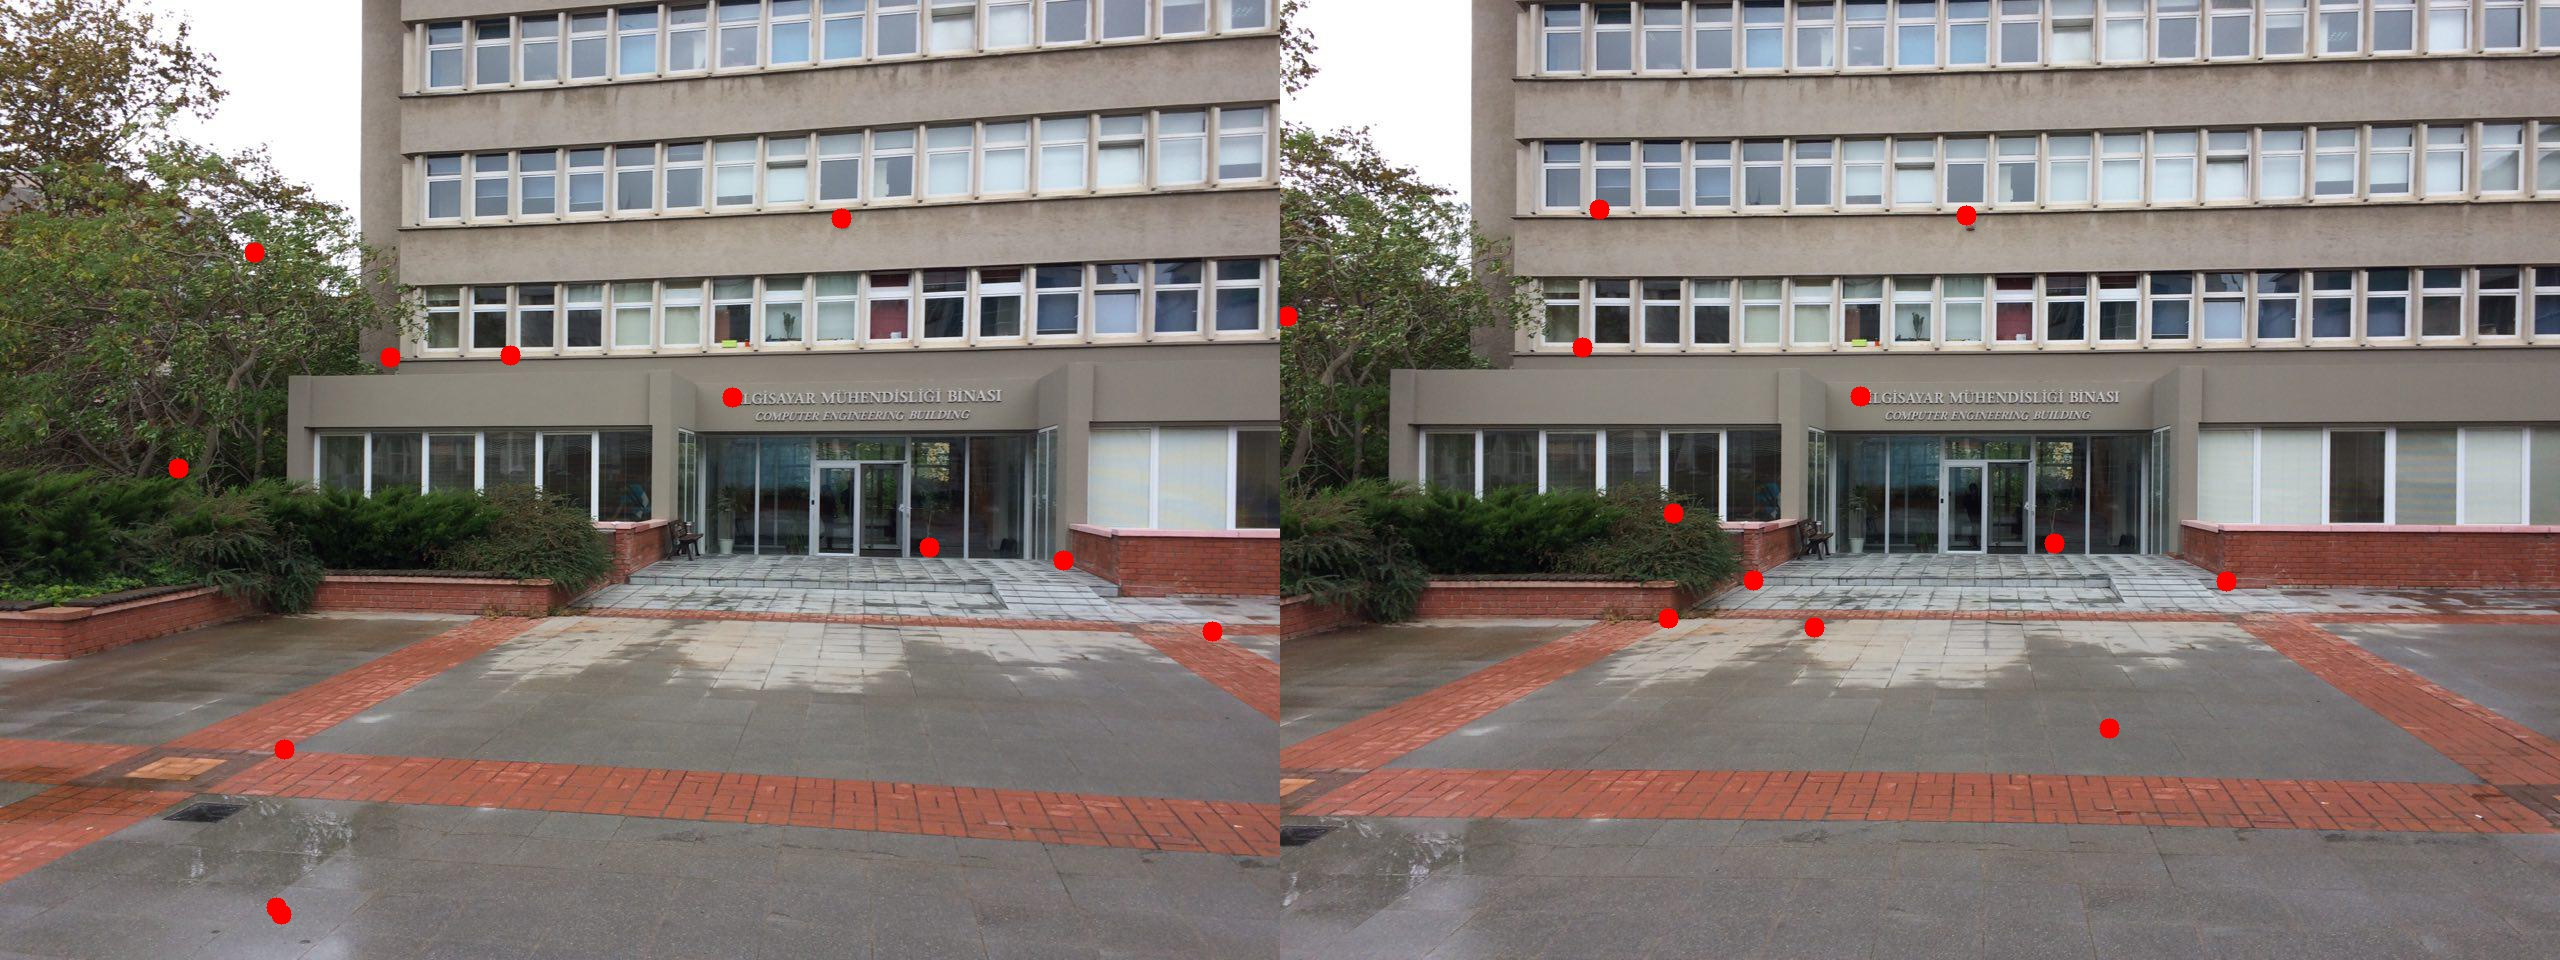
\includegraphics[width=1\columnwidth]{experiments/12points/norm/left-1_middle5wrong.jpg}
          \caption{
                \label{} Common points between left and middle image.
        }
        \centering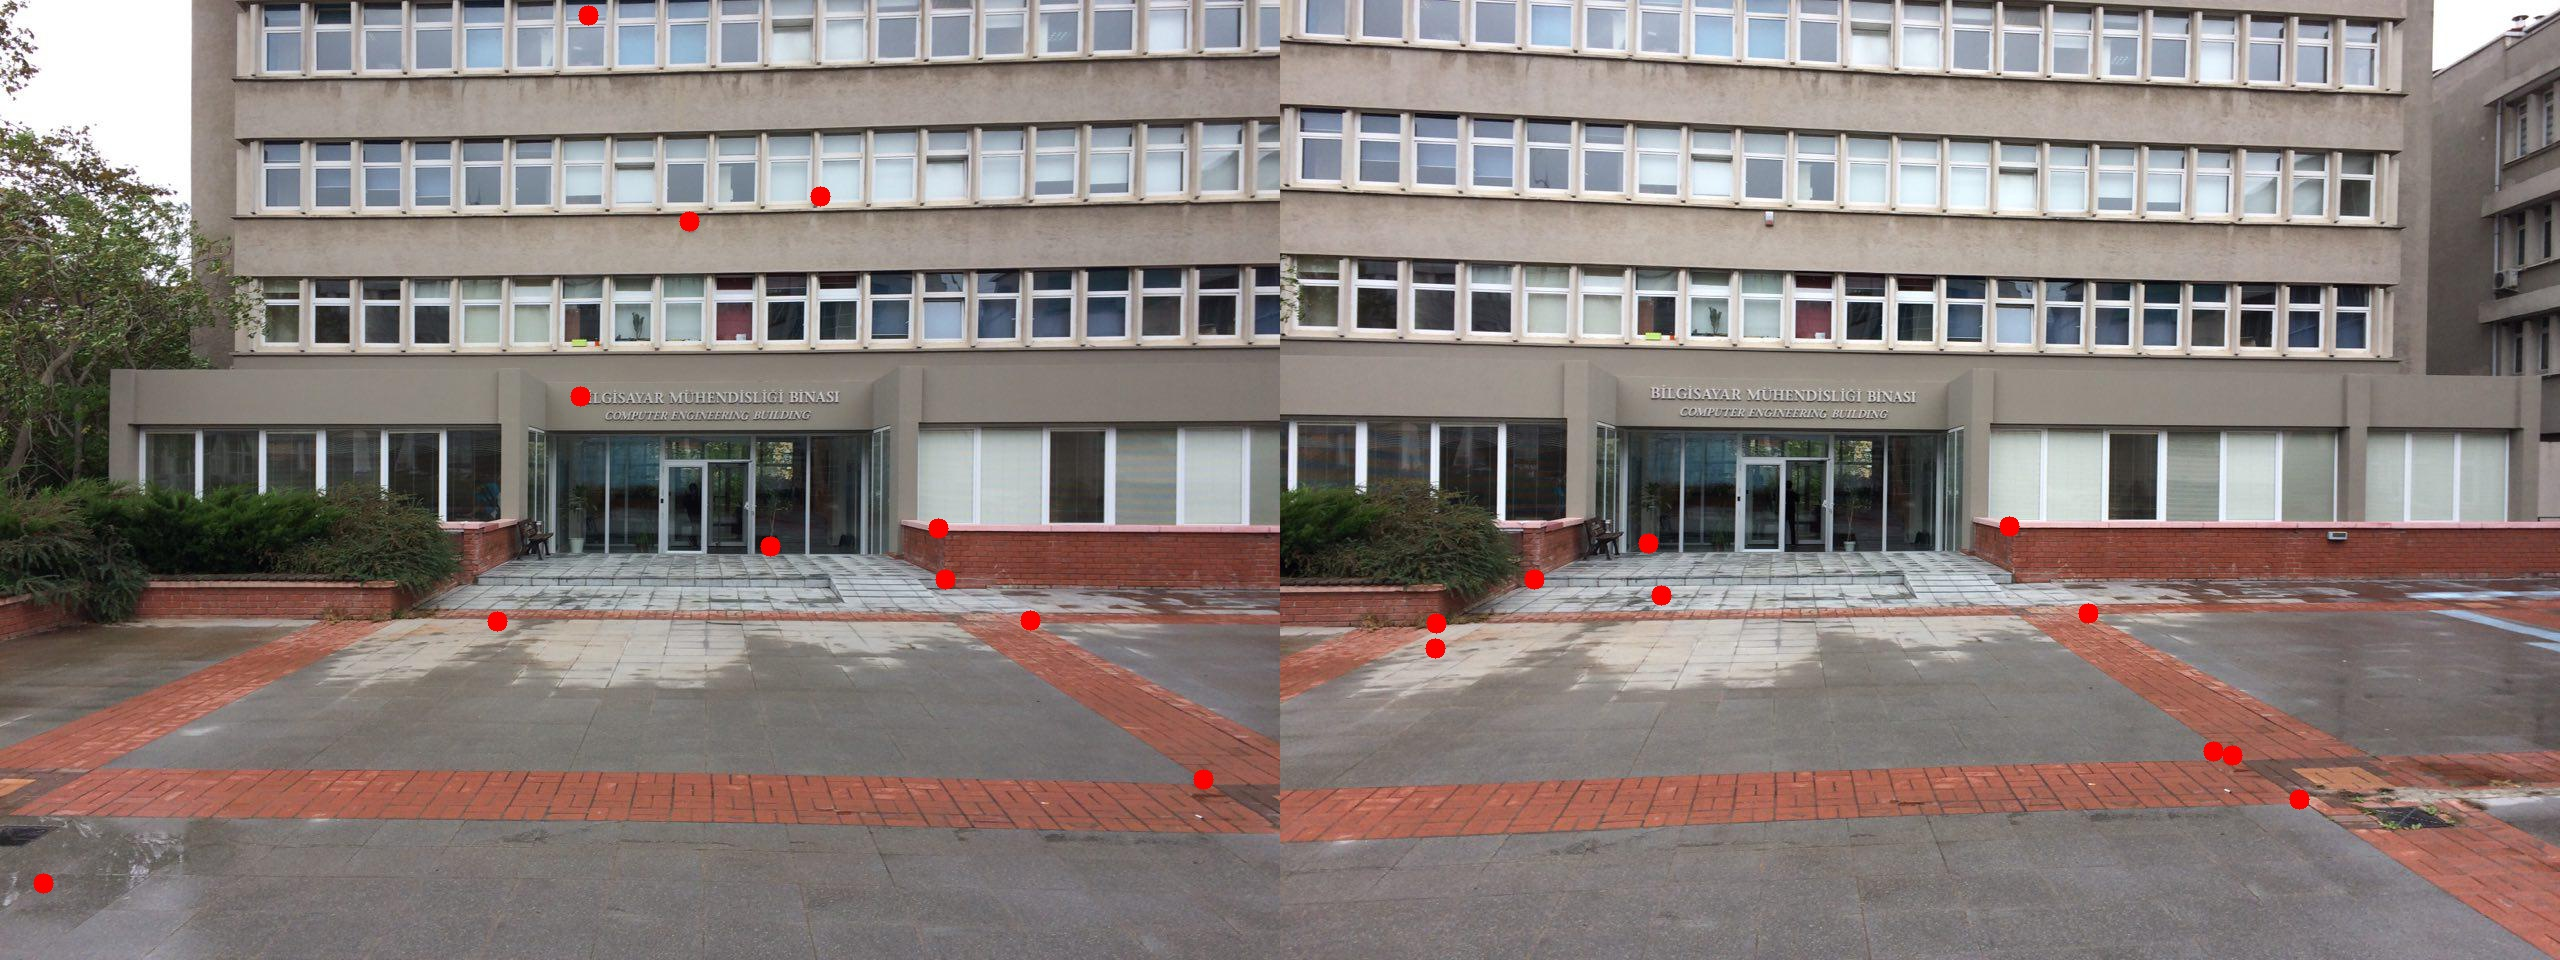
\includegraphics[width=1\columnwidth]{experiments/12points/norm/middle_left-15wrong.jpg}
        \caption{
                \label{} Common points between middle and right image.
        }
\end{figure}
\FloatBarrier
\newpage




\end{document}
